\chapter{Results}
\label{chp:results}

\section{General guidances on interpretation of the results}

To interpret the results one must keep in mind that the estimated coefficients are elasticities. The practical implication of this is that the coefficient values represent the percentual change in the demand for a one percent change in the variable (untransformed to log). Therefore, a coefficient of value $1$ will mean a one percent change in the demand for a one percent change in the predictor variable - fares, GVA or GJT. 

% Another way of stating that is that a coefficient whose value is 1 means that the demand changes proportionally to the change in the predictor variables. When the coefficient is higher than 1 the impact in the demand is more than proportional and, conversely, when it is less, the impact is lower than proportional. Additionally, the proportion of variation above or below the proportional change can, in turn, be stated as a percentage. Thus, for instance, a coefficient whose values is $1.2$ means that the impact in the demand is 20\% more than proportional, and for a coefficient $0.8$, this impact would be 20\% less than proportional.

% Comment on elastic and inelastic

Beyond the point estimates, the Bayesian regression provides a probability density function (pdf) of credible values that the coefficients may assume. In fact, the point estimate is the mean of the posterior distribution. 

An advantage of a pdf output over a point estimate is that it is possible to directly interpret the probabilities of values in a given interval. For instance, one can take two values and compute the probability of the coefficient being in the interval. This is fundamentally different from the frequentist confidence interval, which only regards the probability of a sampling procedure resulting in an interval which contains the true value of the estimated parameter.

The posterior distributions are convenient to discuss the uncertainty of estimates. The usual procedure is taking the high-density interval (HDI) to consider the boundaries of credible values for the coefficients. The HDI is the smallest interval to achieve a given probability, which may differs from the symmetrical density interval, as illustrated by Figure \ref{fig:hdi}, when the distribution is not symmetrical. 

In this work, a HDI of 95\% will be adopted in the analysis. Full information on the estimated HDI is presented on Appendix \ref{apd:bayes_hdi} .

The analysis of the results will be presented with the aid of marginal posterior distribution's plots. This format is useful since it is a bi-dimensional figure, but it worths recovering that the actual posterior distribution, as discussed in Chapter \ref{chp:lit-rev} is a multi-dimensional space, where the dimensions depend on the number of predictor variables.

\begin{figure}
\centering
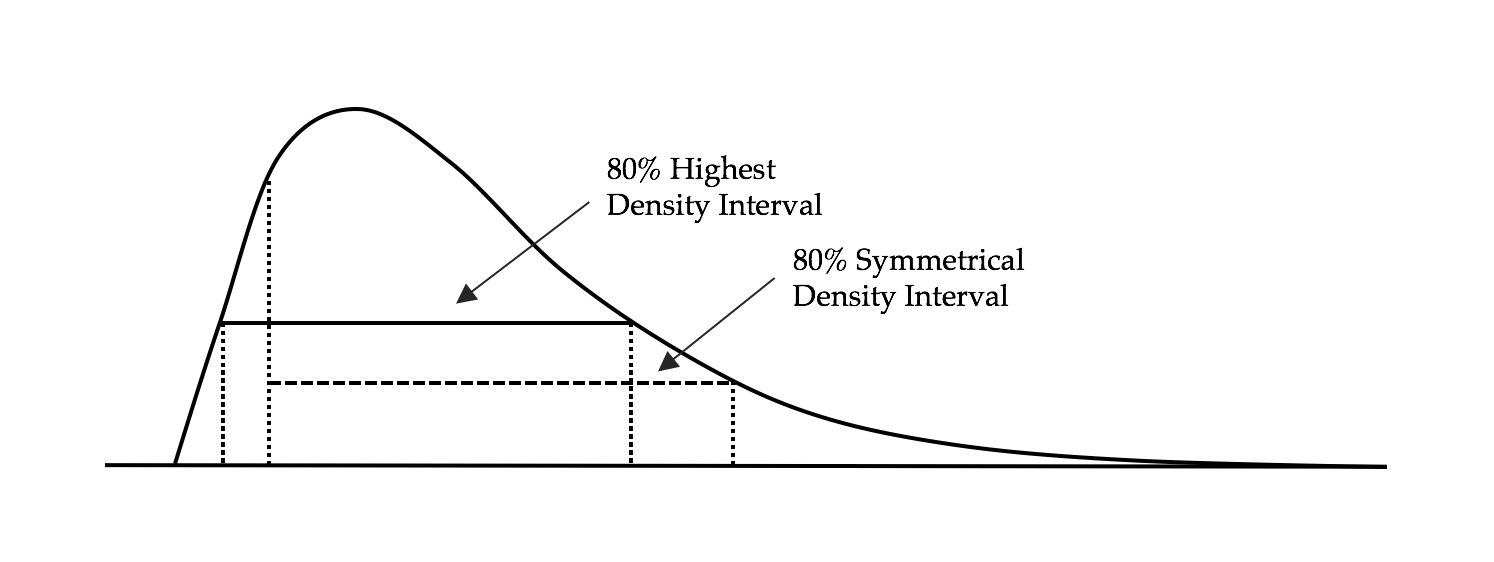
\includegraphics[scale=0.4]{hdi}
\caption{High Density Interval \textit{versus} Symmetrical Density Interval}
\label{fig:hdi}
\caption*{Source: \cite{hdinterval} [adapted]}
\end{figure}

% The advantage of the posterior distribution is that they can be directly interpreted as probabilities in a given interval, which will be useful to discuss the uncertainty around the point estimate. For instance, one can discuss the amplitude of an interval regarding the difference between the lowest and highest values within an HDI. The practical application of analysing the amplitude is measuring how much uncertainty there is between these extreme probable values. Consider, for instance, an elasticity density function whose HDI 95\% is between 1.2 and 1.3. This would mean that the lower probable value of elasticity would be 1.2, which in turn means that demand would vary 20\% for a given percentage change in the predictor, say fare. The highest probable value would be 1.3, which in turn means that demand would vary 30\% for a given percentage change in the same predictor. The conclusion is that there is a small range of values that makes the uncertainty around the elasticity's coefficient varies only 10\%.

An additional consideration when interpreting the posterior distribution plots is that the y axis would eventually be greater than one. This is apparently counter-intuitive since probabilities are defined in the [0,1] domain. However, because it is a continuous function, the actual probability of the estimate assuming a point value is zero. So the y axis should be not be used to directly read the probabilities from values in the x axis. Instead, a probability can only be computed integrating a given an interval. Integrating the full density function it would be approximately 1 \citep{kruschke2014}.

\section{Comparative Estimates: SURE/OLS Models}

For a comparison purpose, frequentist estimates will be provided along the Bayesian estimates. The most plausible approach would be the seemingly unrelated regression estimation (SURE), nevertheless, despite it seems natural to think about the demand estimation for each market as a system of demand equations (one for each type of fare), as taught by \cite{kennedy2003}, SURE estimation becomes identical to OLS when all the predictive variables are the same, which happens to be the case in this study.

The models were estimated based on the linear models presented in Table \ref{tbl:equation_panel}. As it should be expected, the estimation of SURE/OLS models reinforces previous studies showing that ``freely estimating models will not yield robust elasticities" \citep[p.~37]{its-systra-report}. Despite statistically significant - with some exceptions - several estimated elasticities presented unexpected signs, according to the assumptions of the PDFH. Table \ref{tbl:summary_ols} summarises the occurrences. 


\begin{table}[H] \centering 
  \caption{Summary of SURE/OLS outputs with respect to algebraic sign of coefficients} 
  \label{tbl:summary_ols} 
{\renewcommand\arraystretch{1.25}}
\begin{tabular} {cccccc}
\toprule
\multirow{2}{*}{Market} & Dependent & \multicolumn{4}{c}{Elasticities Estimates} \\
\cline{3-6} 
                        & Variable  & \multicolumn{2}{c}{Expected Sign} & \multicolumn{2}{c}{Unexpected Sign} \\
\hline
\multirow{2}{*}{1}      &$ln V_{2F}$& 4 & $f_{2F}$, $f_{2R}$, $g$, $\gamma$                                           & - & - \\
\cdashline{2-6} 
						&$ln V_{2R}$& 3 & $f_{2F}$, $f_{2R}$, $\gamma$                                                & 1 & $g$ \\
\hline
\multirow{3}{*}{2}      &$ln V_{2F}$& 4 & $f_{2F}$, $f_{2A}$, $g$, $\gamma$                                           & 1 & $f_{2R}$ \\
\cdashline{2-6} 
						&$ln V_{2R}$& 4 & $f_{2F}$, $f_{2R}$, $g$, $\gamma$                                           & 1 & $f_{2A}$  \\
\cdashline{2-6} 
						&$ln V_{2A}$& 3 & $f_{2R}$, $f_{2A}$, $g$                                                     & 2 & $f_{2F}$, $\gamma$ \\
\hline
\multirow{4}{*}{3}      &$ln V_{1N}$& 6 & $f_{1N}$, $f_{2F}$, $f_{2R}$, $f_{2A}$, $g$, $\gamma$                       & - & - \\
\cdashline{2-6} 
						&$ln V_{2F}$& 4 & $f_{2F}$, $f_{2A}$, $g$, $\gamma$                                           & 2 & $f_{1N}$, $f_{2R}$ \\
\cdashline{2-6} 
						&$ln V_{2R}$& 4 & $f_{2F}$, $f_{2A}$, $g$, $\gamma$                                           & 2 & $f_{1N}$, $f_{2R}$ \\
\cdashline{2-6} 
						&$ln V_{2A}$& 5 & $f_{2F}$, $f_{2R}$, $f_{2A}$, $g$, $\gamma$                                 & 1 & $f_{1N}$ \\
\hline
\multirow{6}{*}{4}      &$ln V_{1F}$& 8 & $f_{1F}$, $f_{1R}$, $f_{1A}$, $f_{2F}$, $f_{2R}$, $f_{2A}$, $g$, $\gamma$   & - & - \\
\cdashline{2-6} 
						&$ln V_{1R}$& 6 & $f_{1R}$, $f_{2F}$, $f_{2R}$, $f_{2A}$, $g$, $\gamma$                       & 2 & $f_{1F}$, $f_{1A}$ \\
\cdashline{2-6} 
						&$ln V_{1A}$& 6 & $f_{1F}$, $f_{2F}$, $f_{2R}$, $f_{2A}$, $g$, $\gamma$                       & 2 & $f_{1R}$, $f_{1A}$ \\
\cdashline{2-6} 
						&$ln V_{2F}$& 3 & $f_{2A}$, $g$, $\gamma$                                                     & 5 & $f_{1F}$, $f_{1R}$, $f_{1A}$, $f_{2F}$, $f_{2R}$    \\
\cdashline{2-6} 
						&$ln V_{2R}$& 8 & $f_{1F}$, $f_{1R}$, $f_{1A}$, $f_{2F}$, $f_{2R}$, $f_{2A}$, $g$, $\gamma$   & - & - \\
\cdashline{2-6} 
						&$ln V_{2A}$& 7 & $f_{1F}$, $f_{1A}$, $f_{2F}$, $f_{2R}$, $f_{2A}$, $g$, $\gamma$             & 1 & $f_{1R}$ \\
\bottomrule
\end{tabular}%
\caption*{Source: Own work}
\end{table} 

% \textit{GVA}      &\multicolumn{2}{m{6cm}}{\raggedright regional GVA, at NUTS 3 level, in millions of pounds, 2014 values.} 

\section{Bayesian models with weakly informative priors}

Because it is safer to estimate Bayesian models gradually building in complexity, Bayesian models with weakly informative priors were estimated before the constrained models. The priors established for these models have followed the same guidances from Chapter \ref{chp:methods}, but without the truncation.

The models were run without any issues. However, this estimation was of little help in generating estimates with correct algebraic signs resulting in estimates very similar to the OLS. This may be explained due to the high volume of data that makes the likelihood prevails over the prior distribution \citep{kruschke2014}. Therefore, the valuable prior information added to the models was the restriction applied in the domain of the elasticities' probability densities, as discussed in the next section.

For completeness, the Appendix \ref{apd:bayes_weakpriors} presents the results of estimated models with weakly informative priors. 

\section{Bayesian constrained models}

\subsection{Market 1}

\textit{i. Autocorrelation and convergence}

The first market, with only two fares competing, is the simpler one. The model converged with low autocorrelation in the posterior samples, as shown by the statistics in Table \ref{mkt1_T_autocorr_convergence}.

% latex table generated in R 3.3.2 by xtable 1.8-2 package
% Sat Aug  5 10:10:51 2017
\begin{table}[ht]
\caption{Autocorrelation and convergence measures - Market 1}
\label{mkt1_T_autocorr_convergence}
\centering
\begin{tabular}{lrrrrr}
\toprule 
 & \multicolumn{5}{c}{\textit{Dependent variable:}} \\ 
\cline{2-6} 
\\[-1.8ex] & \multicolumn{2}{c}{$ln \; V_{2F}$} & & \multicolumn{2}{c}{ $ln \; V_{2R}$}\\ 
\cline{2-3} \cline{5-6}
 & $\hat{R}$ & $n_{\text{eff}}$ & &$\hat{R}$ & $n_{\text{eff}}$ \\ 
  \midrule

  $f_{2F}$ & 1.0 & 1650 & & 1.0 & 402 \\ 
  $f_{2R}$ & 1.0 & 1692 & & 1.0 & 821 \\ 
  $g$      & 1.0 & 1561 & & 1.0 & 719 \\ 
  $\gamma$ & 1.0 & 1778 & & 1.0 & 432 \\ 
  Constant & 1.0 & 1477 & & 1.0 & 702 \\ 
   \hline
   Iter    & \multicolumn{2}{c}{2,000} && \multicolumn{2}{c}{2,000} \\
   Thin    & \multicolumn{2}{c}{1} && \multicolumn{2}{c}{1} \\
   \bottomrule
\end{tabular}
\caption*{Source: Own work}
\end{table}

It is relevant, however, to consider that a warning of divergent transitions after the warm-up was reported for both regressions. The issue around it is that these warnings signalise that the estimates might be biased \citep{stan_warnings}, even though they have converged to stable and equivalent variances across the chains.

The divergent transitions are likely to be related to the imposition of constraints in the domain of the probability density. This might have prevented the MCMC to explores the parameter space with plausible values according to the likelihood, but constrained by the prior. Therefore, it appears that the divergent transitions are part of the adopted solution of applying restrictions to prevent unfeasible estimates.

It will be assumed, therefore, that biased estimates are the best information at hand and should not be discarded. As taught by \cite{gelman_blog}, in the context of Bayesian data analysis, one should recognise that ``unbiasedness" is a very idealistic concept, and because it may hardly be achieved, one should not refrain oneself to make usage of the available information.
\\[3pt]

\textit{ii. OLS comparison}

A comparison between the Bayes and OLS estimates is presented in Table \ref{tbl:mkt1_T}. As expected, the all Bayesian coefficients have coherent signs. It has clearly improved the estimation of $g$ with respect to the $V_{2R}$ demand, for which the OLS estimation has failed.

% In general terms, it is possible to say that no big discrepancies were observed from the two estimates and their respective standard deviations, excepted for the $g$ parameter. This is easier to see with the aid of the Figures ahead.

% latex table generated in R 3.3.2 by xtable 1.8-2 package
% Mon Jul 31 09:29:49 2017
\begin{table} [H]
\caption{Comparison of bayesian and SURE/OLS estimates - Martket 1}
\label{tbl:mkt1_T}
\centering
\begin{tabular}{rrrrrrrrrrr}
  \toprule 
 & \multicolumn{2}{c}{\textit{Bayes}} & & \multicolumn{2}{c}{\textit{SURE/OLS}} \\ 
\cline{2-3} \cline{5-6}
\\[-1.8ex] & $ln \; V_{2F}$ & $ln \; V_{2R}$ & & $ln \; V_{2F}$ & $ln \; V_{2R}$ \\ 
\hline \\[-1.8ex] 

  $f_{2F}$ & -1.32 & 0.70 & &-1.28 & 0.81\\
  		   & (0.05)  & (0.05) & & (0.05) & (0.05)\\ [0.2cm]
  $f_{2R}$ & 0.17 & -0.89  & & 0.17 & -0.89 \\
  			& (0.05) &  (0.05) & & (0.05) & (0.05)\\ [0.2cm]
  $g$ & 0.77 & 0.06 & & 0.49 & \cellcolor{gray!25}-0.52 \\
  		& (0.05) & (0.04) & & (0.7) & (0.7)\\ [0.2cm]
  $\gamma$ & -0.89 & -0.88 & & -0.98 & -1.06\\
  			& (0.04) & (0.05) & & (0.04) & (0.05)\\ [0.2cm]
  Constant & 6.10 & 11.27 & & 9.14 & 17.6\\
  			& (0.57) & (0.47) & & (0.71) & (0.73)\\ [0.2cm]
  % \hline
  % $\sigma$ & 1.43 & 1.48 & & -& -\\
  % 		 & (0.01) & (0.01) & & -& -\\
\bottomrule
\end{tabular}
\caption*{Source: Own work}
\end{table}


\textit{iii. Uncertainty}

% 1.
Figures \ref{fig:mkt1_v2f_post} and \ref{fig:mkt1_v2r_post} present the marginal posterior distribution of the estimated elasticities coefficients. The continuous lines represent the Bayesian mean, the red line represents the OLS mean and the dotted lines represent the boundaries of the 95\% HDI.

% 2.
As one may notice, the small standard deviations are reflected in a posterior distribution with a decimal scale for all estimates, except the constant - which usually will not be covered in the analysis. These small ranges of credible values for the coefficients are useful since these are elasticities measures. It is important that they do not allow the distribution to spread much, becoming low-quality information. 

This is also reflected in the HDI boundaries, which are very close to the mean value demonstrating that there is a small range of credible values. As a general rule, it will be considered that an HDI up 0.30 is satisfactorily small. Above this value, the uncertainty would be unfavourable to any practical application since this decimal variation in the coefficient, in fact, is a percent impact on the demand. Detailed information of the HDI is presented in the Appendix \ref{apd:bayes_hdi}. 

% 3ab.
With respect to the $V_{2f}$ demand, Figure \ref{fig:mkt1_v2f_post}, all elasticities distributions are smooth bell-shaped curves, demonstrating that they have not faced any strong constraint. Indeed, the OLS estimate already had the correct signs, so there was no conflict in the estimation.

% 3c.
Even though the OLS estimates had correct signs, some of them were not considered credible values according to the Bayesian estimation: the $g$ elasticity lied out of the HDI and the $\gamma$ was at the edge. 

\begin{figure}[H]
\centering
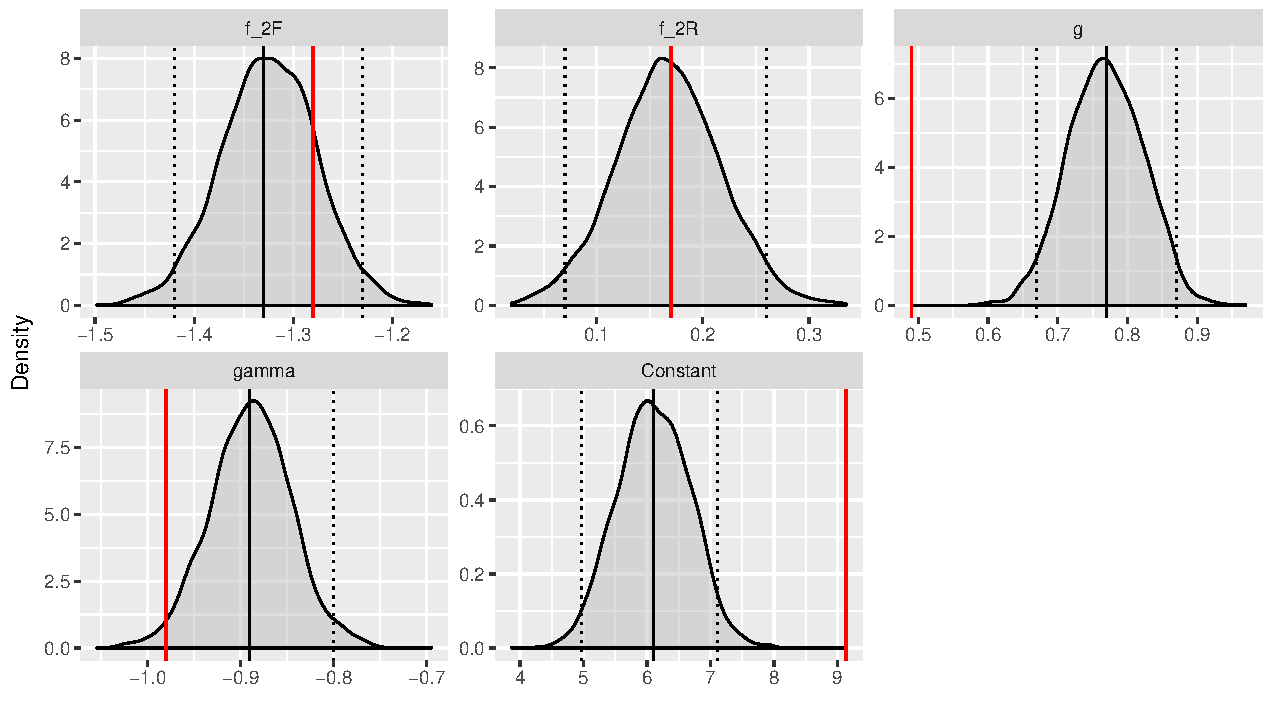
\includegraphics[width=\linewidth]{mkt1_v2f_post.pdf}
\caption{Posterior density function of elasticities w.r.t $V_{2F}$ - Market 1}
\label{fig:mkt1_v2f_post}
\caption*{Source: Own work}
\end{figure} 

% 3a.
With respect to the $V_{2R}$ demand, Figure \ref{fig:mkt1_v2r_post}, the curves are bell-shaped, except for the $g$ which is skewed towards the left. It is noticeable that this is the sign-reverted elasticity. It appears that the constraint at zero, which blocked the distribution to assume negative values, was an actual barrier. Indeed this may explain the warnings of divergent transitions.

% 3b.
All HDI were satisfactorily small, from 0.14 to 0.20. 

% 3c.
The OLS estimates of $f_{2F}$, $g$ and $\gamma$ are out of the HDI, demonstrating that these are not credible values according to the Bayesian estimation. Opposedly, the OLS estimate for $f_{2R}$ was coincident. 

\begin{figure}[H]
\centering
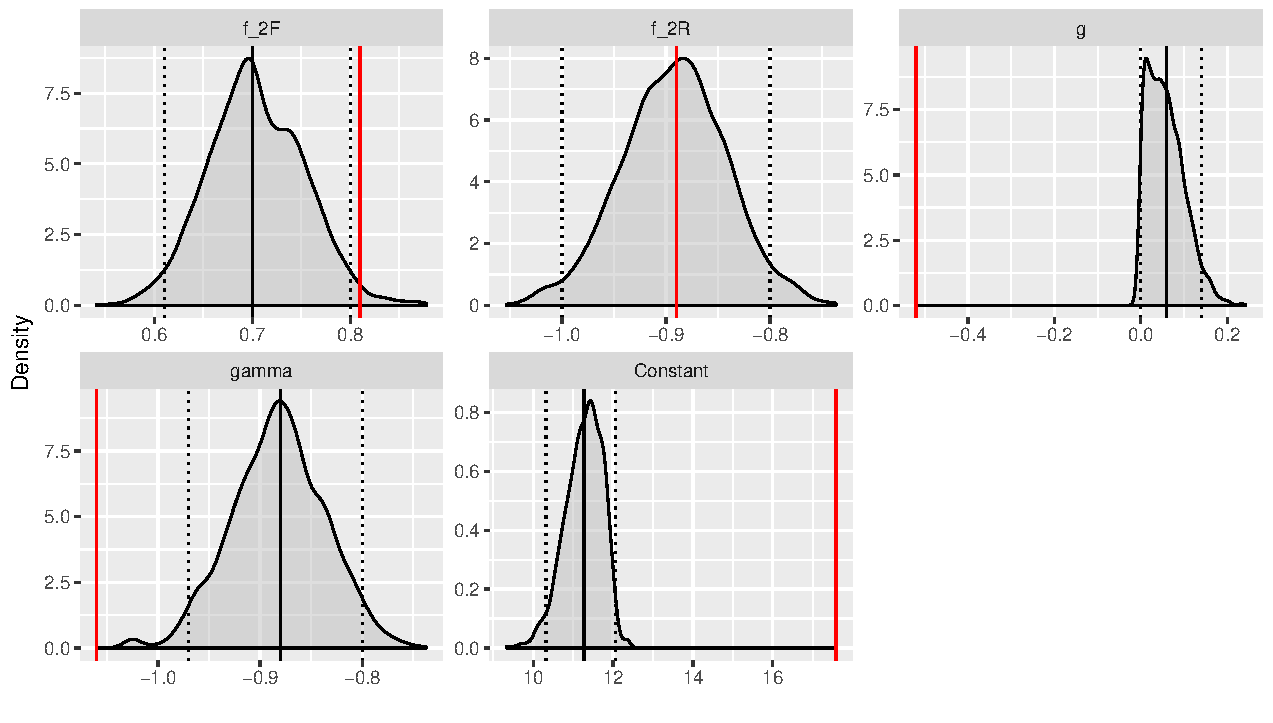
\includegraphics[width=\linewidth]{mkt1_v2r_post.pdf}
\caption{Posterior density function of elasticities w.r.t  $V_{2R}$ - Market 1}
\label{fig:mkt1_v2r_post}
\caption*{Source: Own work}
\end{figure} 

\textit{iv. Magnitude of estimates}

Analysing the magnitude and distributions of coefficients one can notice that the \textit{Full} fare is more sensitive to its own price, with mean -1.3, then the \textit{Reduced} fare, with mean -0.9. This difference may be reasonable if one considers the \textit{Reduced} fare as a basic service, accessible for everyone without time restrictions, whilst the \textit{Full} fare would offer a plus of convenient schedules in the peak hours. The price differentiation of \textit{Reduced} and \textit{Full} and its different sensitiveness to price would, therefore, be in accordance with economic theory which says that superfluous goods are more elastic than essential goods.

The magnitude of cross elasticities can be also interpreted by this rationale of basic and more convenient services. Therefore, the demand of \textit{Reduced} fare is more affected by variations in the price of the \textit{Full} fare than the contrary, which means that everything constant, when the \textit{Full} fare increases more passenger change for the \textit{Reduced} fare than vice-versa.

In which regards the GVA elasticity it is unexpectedly below 1 for the demand of \textit{Full}, with mean 0.7, and even more unexpected for the demand of \textit{Reduced}, being very close to zero. According to the PDFH, the GDP elasticities - for which GVA is assumed as an equivalent measure of income/wealth \citep[p.~ 4, Chapter B1]{pdfhv5}, are expected to be around $1.1$ \citep[p.~9, Chapter B1]{pdfhv5}. 

Irrespective of their magnitude, the fact that $g_{2F} > g_{2R}$ should be expected because there is a higher proportion of business trips in the \textit{Full} fare than in the \textit{Reduced}, for non-London long distance journeys \citep{pdfhv5}.

Lastly, the quality elasticity was very similar in both \textit{Full} and \textit{Reduced} demands, with mean -0.9 and similar standard deviation. These values are within the expected interval of -0.7 to -1.1, according to the PDFH \citep{pdfhv5}. However, business travellers are more sensitive to quality rather than price because ``it is undertaken at the time and at the expense of the employer" \citep[p.~1, Chapter A1]{pdfhv5}. Because of that, $\gamma_{2F} > \gamma_{2R}$ should be expected, which was not observed. 

% ====================================
% ====================================
% ====================================

\subsection{Market 2}

\textit{i. Autocorrelation and convergence}

In Market 2, the estimation was more complex. Both the $V_{2R}$ and $V_{2A}$ regressions demanded longer iterations (10,000 instead of 2,000) to converge with an acceptable amount of effective samples. Nevertheless, the estimation was successful, as demonstrated by the statistics in Table \ref{mkt2_T_autocorr_convergence}.

As in Market 1, there also were divergent transitions reported in all three regressions of Market 2. The previous interpretation applies.
% \\[3pt]

% latex table generated in R 3.3.2 by xtable 1.8-2 package
% Sat Aug  5 10:10:51 2017
\begin{table}[H]
\caption{Autocorrelation and Convergence Measures - Market 2}
\label{mkt2_T_autocorr_convergence}
\centering
\begin{tabular}{lrrrrrrrr}
\toprule 
 & \multicolumn{8}{c}{\textit{Dependent variable:}} \\ 
\cline{2-9} 
\\[-1.8ex] & \multicolumn{2}{c}{$ln \; V_{2F}$} & & \multicolumn{2}{c}{ $ln \; V_{2R}$} & &  \multicolumn{2}{c}{ $ln \; V_{2A}$}\\ 
\cline{2-3} \cline{5-6} \cline{8-9}
 & $\hat{R}$ & $n_{\text{eff}}$ & & $\hat{R}$ & $n_{\text{eff}}$  & & $\hat{R}$ & $n_{\text{eff}}$ \\ 
\hline \\[-1.8ex] 
  $f_{2F}$ & 1.0 & 405 & & 1.0 & 464 & & 1.0 & 529 \\ 
  $f_{2R}$ & 1.0 & 251 & & 1.0 & 414 & & 1.0 & 493 \\ 
  $f_{2A}$ & 1.0 & 614 & & 1.0 & 702 & & 1.0 & 634 \\ 
  $g$      & 1.0 & 315 & & 1.0 & 561 & & 1.0 & 555 \\ 
  $\gamma$ & 1.0 & 400 & & 1.0 & 525 & & 1.0 & 912 \\ 
  Constant & 1.0 & 310 & & 1.0 & 548 & & 1.0 & 500 \\
   \hline
   Iter    & \multicolumn{2}{c}{2,000} && \multicolumn{2}{c}{10,000} && \multicolumn{2}{c}{10,000} \\
   Thin    & \multicolumn{2}{c}{1} && \multicolumn{2}{c}{1} && \multicolumn{2}{c}{1} \\
   \bottomrule
\end{tabular}
\caption*{Source: Own work}
\end{table}


\textit{ii. OLS comparison}

A comparison between the Bayes and OLS estimates is presented in Table \ref{tbl:mkt2_T}. As expected, the all Bayesian coefficients have coherent signs. It has clearly improved the estimates since the OLS present four wrong sign elasticities.
% \\[3pt]

% latex table generated in R 3.3.2 by xtable 1.8-2 package
% Mon Jul 31 09:29:49 2017
\begin{table} [H]
\caption{Comparison of bayesian and SURE/OLS estimates - Martket 2}
\label{tbl:mkt2_T}
\centering
\begin{tabular}{rrrrrrrrrrr}
  \toprule 
 & \multicolumn{3}{c}{\textit{Bayes}} && \multicolumn{3}{c}{\textit{SURE/OLS}} \\ 
\cline{2-4} \cline{6-8} 
\\[-1.8ex] & $ln \; V_{2F}$ & $ln \; V_{2R}$ & $ln \; V_{2A}$ & & $ln \; V_{2F}$ & $ln \; V_{2R}$ & $ln \; V_{2A}$ \\ 
\hline \\[-1.8ex] 

  $f_{2F}$ & -1.29  & 0.04   & 0.05 & & -1.24 & 0.03$^{\dagger}$ & \cellcolor{gray!25}-0.18\\
  		     & (0.05) & (0.03) & (0.04) & & (0.06) & (0.06) & 0.10)\\ [0.2cm]
  $f_{2R}$ & 0.05   & -0.80  & 1.01 & &\cellcolor{gray!25}-0.06 & -0.60 & 1.03\\
  			   & (0.04) & (0.05) & (0.08) & & (0.08) & (0.08) & (0.13)\\ [0.2cm]
  $f_{2A}$ & 0.14   & 0.01   & -0.46 & &0.15 & \cellcolor{gray!25}-0.10 & -0.47 \\
           & (0.04) & (0.01) & (0.06) & &(0.04) & (0.04) & (0.06)\\ [0.2cm]
  $g$      & 1.68   & 0.96   & 0.29  & &1.75 & 0.39 & 0.66\\
  		     & (0.07) & (0.07) & (0.08) & &(0.11) & (0.10) & (0.17)\\ [0.2cm]
  $\gamma$ & -1.28  & -1.07  & -0.03 & &-1.23 & -1.21 & \cellcolor{gray!25}0.33\\
  			   & 0.06   & (0.06) & (0.03) & &(0.07) & (0.06) & (0.10)\\ [0.2cm]
  Constant & -0.28  & 5.46   & -0.61 & &-1.09$^{\dagger}$ & 11.72 & -5.53\\
  			   & (0.76) & (0.71) & (0.82) & &(1.15) & (1.09) & (1.77)\\ [0.2cm]
  % \hline
  % $\sigma$ & 1.36  & 1.29   & 2.10 &&&&\\
  % 		     & (0.01)& (0.01) & (0.02)&&&&\\
\bottomrule
Note: $^{\dagger}$ $p>0.1$
\end{tabular}
\caption*{Source: Own work}
\end{table}





% Additionally, it is possible to notice that the estimates, when not corrected, were very close to the OLS values, except for the GVA elasticities in the $ln V_{2R}$ and $ln V_{2A}$ regressions. The same is valid for the standard deviations. That may indicate that the constraints in the probability density functions' domains are being effective to estimate a coherent elasticity coefficient. To the other coefficients, the likelihood, which has similar results to the SURE/OLS estimates, prevails given the high number of observations.

\textit{iii. Uncertainty}

% 1.
Figures \ref{fig:mkt2_v2f_post}, \ref{fig:mkt2_v2r_post} and \ref{fig:mkt2_v2a_post} illustrate the probability densities of the estimated elasticities coefficients. The elements in the graphs remain as explained for Market 1.

% 2.
Again, the small standard deviations were very important in constraining the range of credible values for the estimates in the decimal, even centesimal, scale. The HDI was generally satisfactorily small with the exception of two elasticities, with respect the demand $V_{2A}$. Nevertheless, they were very close to 0.30.

% 3a.
With respect to the $V_{2F}$ demand, Figure \ref{fig:mkt2_v2f_post}, all HDI were in generally satisfactorily small, from 0.14 to 0.28, demonstrating low uncertainty since the credible values are concentrated in small intervals. It is observed that the fare elasticities had the smaller HDI - 0.17, 0.14 and 0.15 for \textit{Full}, \textit{Reduced} and \textit{Advance}, respectively, in opposition to the $g$ and $\gamma$ which were above 0.20. Detailed information of the HDI is presented in the Appendix \ref{apd:bayes_hdi}. 

% 3b.
The OLS estimates lied inside the HDI interval, which indicates that the OLS estimates can be deemed credible values according to the Bayesian estimation. An exception is made for the $f_{2R}$, for which it should already be expected since its OLS estimate was on an unfeasible domain. 

% 3c.
All elasticities distributions are bell-shaped curves, although with some deformity, except for the $f_{2R}$, skewed towards the left with an abrupt cut at zero. It is noticeable that this is the sign-reverted elasticity, which may indicate that the constraint to a positive domain was an actual barrier. What apparently happens is that, because the likelihood considers feasible values on the negative side but the prior does not allow this domain, they tend to agree until zero, so samples are extracted until the limit of the constraint. Beyond that point, they clash, and since the prior assumes zero probability for those values, it is reflected in the posterior distribution. Indeed this may explain the warnings of divergent transitions. 

\begin{figure}[H]
\centering
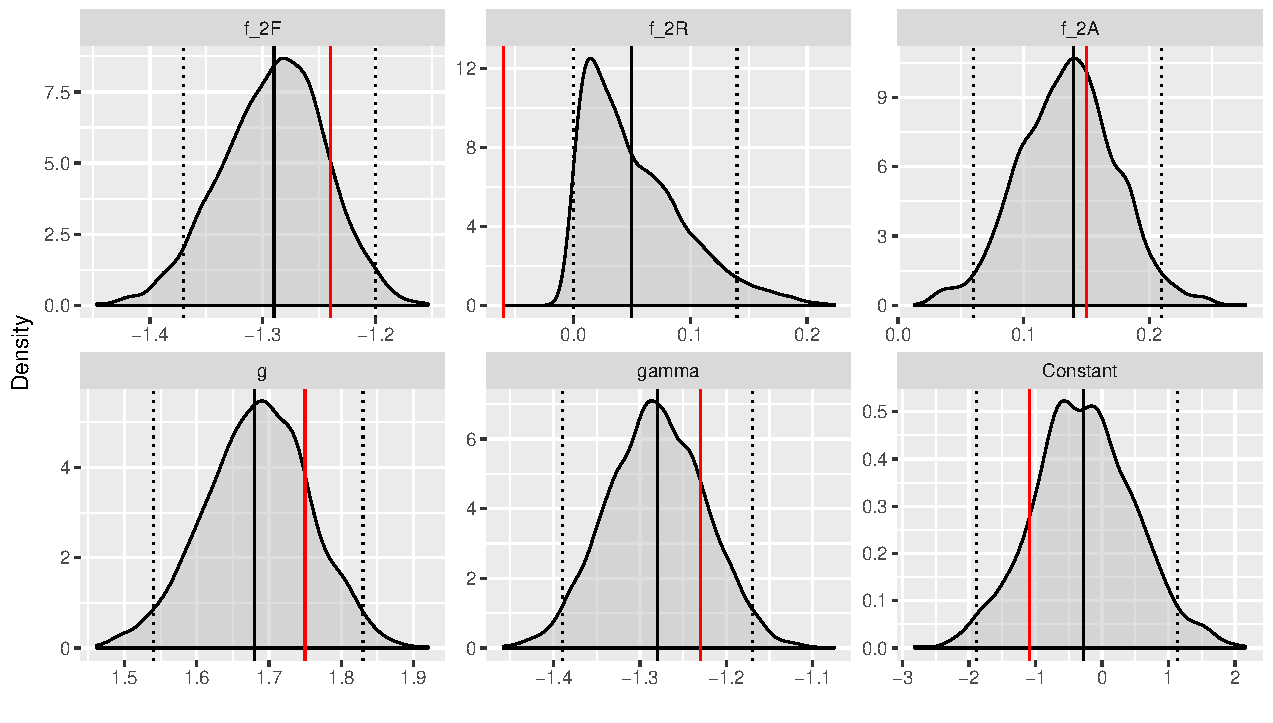
\includegraphics[width=\linewidth]{mkt2_v2f_post.pdf}
\caption{Posterior density function of elasticities w.r.t $V_{2F}$ - Market 2}
\label{fig:mkt2_v2f_post}
\caption*{Source: Own work}
\end{figure} 

% 3a.
With respect to the demand $V_{2R}$, Figure \ref{fig:mkt2_v2r_post}, there were very short HDI intervals, as for $f_{2F}$ and $f_{2A}$, 0.09 and 0.03 respectively, indicating a very precise estimation. The other fare elasticity can also be considered with low HDI, ranging 20\%. Again the $g$ and $\gamma$ had higher intervals. Detailed information of the HDI is presented in the Appendix \ref{apd:bayes_hdi}. 

% 3b.
The OLS estimation lied inside the HDI interval only for the $f_{2F}$ elasticity, which indicates big discrepancies between the Bayesian and frequentist's outputs.

% 3c.
Again, the sign-reversed coefficient, $f_{2A}$, had its distribution finishing abruptly at the zero bound. The cut at zero also appears for the $f_{2F}$ elasticity. Here it is also applied the interpretation of the sharp edge made for the $f_{2R}$, with respect to the demand $V_{2F}$.

\begin{figure}[H]
\centering
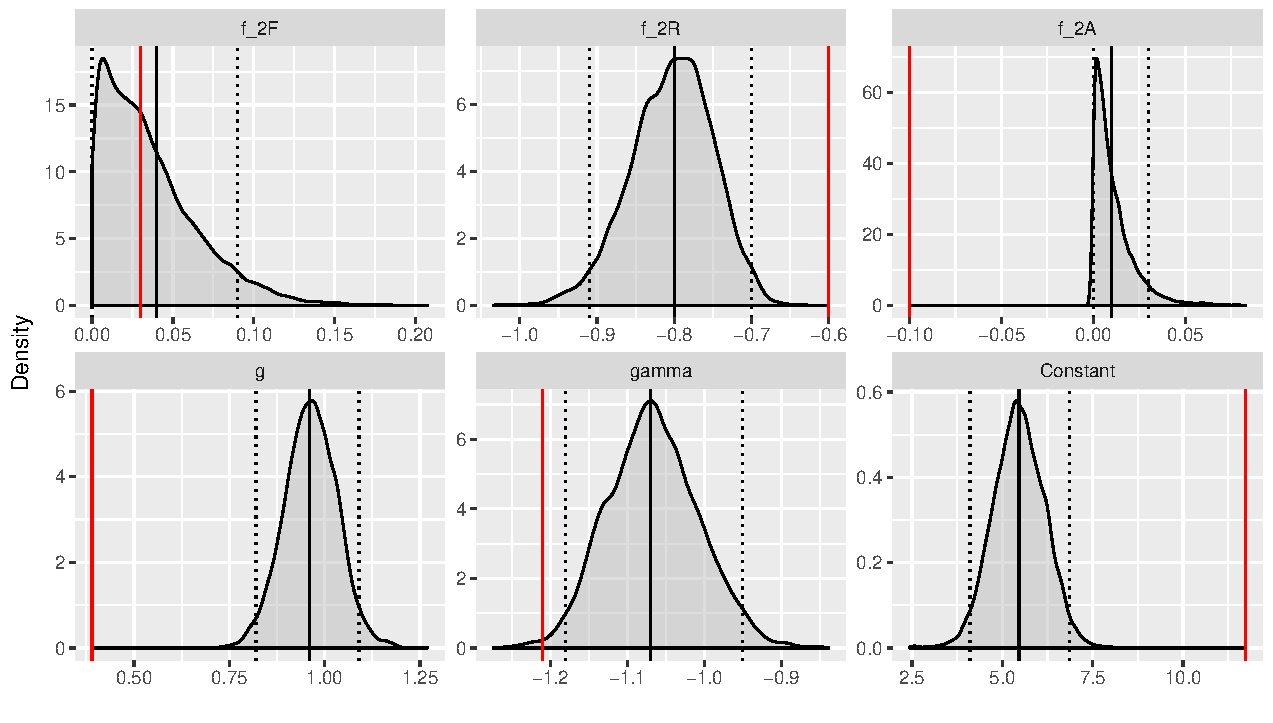
\includegraphics[width=\linewidth]{mkt2_v2r_post.pdf}
\caption{Posterior density function of elasticities w.r.t $V_{2R}$ - Market 2}
\label{fig:mkt2_v2r_post}
\caption*{Source: Own work}
\end{figure} 

% 3a.
With respect to the demand $V_{2A}$, Figure \ref{fig:mkt2_v2a_post}, the HDI's range was satisfactorily small for $f_{2F}$, $f_{2A}$ and $\gamma$, with a surprisingly precise estimate ranging only 0.08. For the other elasticities, however, they were above 0.30, even though they are close to it. It must be highlighted that one can always trade-off certainty for precision, which means that reducing the target probability of HDI will also provide more precise intervals. Detailed information of the HDI is presented in the Appendix \ref{apd:bayes_hdi}. 

% 3b
The analysis of the position of OLS estimates relatively to the HDI shows divergences between the two estimation methods. Only for $f_{2R}$ and $f_{2A}$ the OLS mean lies inside the HDI.

% 3c
Again, the sign-reversed coefficients, $f_{2F}$ and $g$ presented a sharp edge at the zero value. The previous interpretation applies.

\begin{figure}[H]
\centering
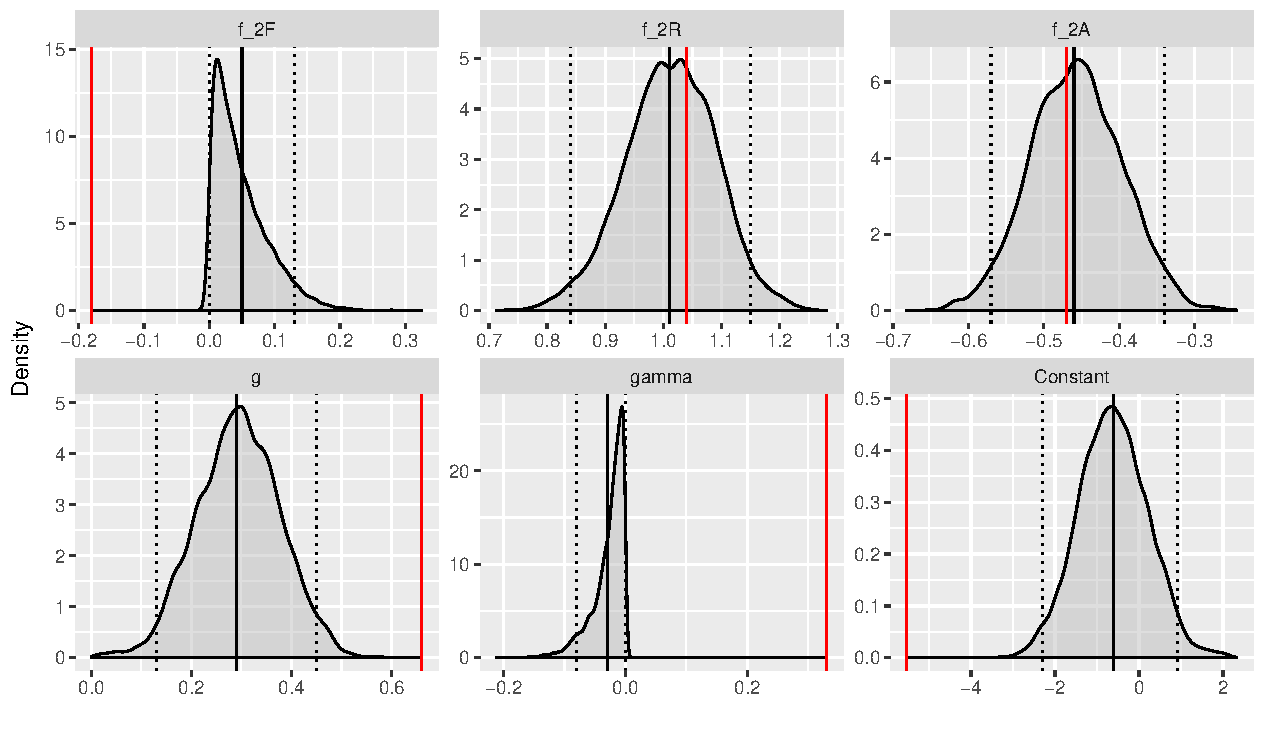
\includegraphics[width=\linewidth]{mkt2_v2a_post.pdf}
\caption{Posterior density function of elasticities w.r.t $V_{2A}$ - Market 2}
\label{fig:mkt2_v2a_post}
\caption*{Source: Own work}
\end{figure} 

% \\[3pt]

\textit{iv. Magnitude of estimates}

% 1.
Analysing of the magnitude of coefficients, the most sensitive fare with regard its own price is \textit{Full}, with mean -1.29, followed by the \textit{Reduced}, with mean -0.80. These values are close to the estimates in Market 1, which is interesting since both do not have \textit{First Class} tickets. The \textit{Advance} fare presented a lower own elasticity, -0.46.

% 2.
Regarding the cross elasticities, for the \textit{Full} fare they were very small - 0.04 and 0.05, indicating a very low impact in the other ticket demands. 

Conversely, for the \textit{Reduced}, a notably high cross elasticity of 1.01 - higher than the own elasticity, was computed with respect to the \textit{Advance} demand. The other cross elasticity was a very small effect - -0.05.

Lastly, for the \textit{Advance} fare, both cross elasticities were considerably small effects - 0.014 and 0.01.

% % these high cross elasticities of $f_{2R}$ with respect the demand of 2A tickets may be justified because reduced demand is more related to leisure passengers [CITE SOMETHING], they are more willing to adapt behaviour if necessary. Therefore, facing an increase in prices, a passenger will plan their trips in advance - which causes the migration to the 2A  demand. Conversely, if prices go down, there is no value in committing themselves with anticipated plans of a trip. 

% % If the volume of \textit{Reduced} tickets were equivalent to the volume of \textit{Advance} one should expect the $f_{2A}$ coefficient in the $ln V_{2R}$ regression to be equivalent, however, as long as the \textit{Advance} tickets are quota controlled... (see also market share of tickets). [IS IT TRUE? SEE SLUTISKY SIMMETRY].

% 3.
The GVA elasticity in this market are significantly higher than in the Market 1, which is difficult to interpret. However, a sign of consistency is noticed since there still is the pattern of the GVA affecting more the \textit{Full} demand, whose mean is 1.68, then the \textit{Reduced}, whose mean is 0.96. For the \textit{Advance} demand the elasticity was of 0.29, but because the advance fares are a mix of promotional fares from both \textit{Full} and \textit{Reduced} it is difficult to interpret it as well.

% 4.
Lastly, the GJT elasticities were also higher than in Market 1, which is difficult to reasonably interpret. Additionally, they did not follow the same pattern from the previous market, in which they coefficients had very similar means. Instead, for the \textit{Full} demand the mean was deemed as -1.28, and for the \textit{Reduced} it was -1.07.

It is interesting, however, that the GJT elasticity of the \textit{Advance} ticket has a very tight distribution close to zero, being far from the expected interval of -0.7 and -1.1 \citep{pdfhv5} without an explicit reason.

% can be interpreted due to the nature of that fare. Because it is a mix of promotional fares from both \textit{Full} and \textit{Reduced} passengers are not sensitive to the quality of the service, since buying an advanced ticket is only a matter of discount for experiencing either one or other service. 
% ==================================
% ==================================
% ==================================

\subsection{Market 3}

\textit{i. Autocorrelation and convergence}

In the third market, the estimation was more complex than in previous markets. The estimation of $V_{2F}$, $V_{2R}$ and $V_{2A}$ demanded longer iterations (10,000 instead of 2,000) to converge with an acceptable amount of effective samples. Additionally, to reduce autocorrelation, the thinness was increased to 5. The resultant estimation was successful, with low autocorrelation, as shown in Table \ref{mkt3_T_autocorr_convergence_SCOTYORK}.

As in Market 1 and 2, there also were divergent transitions reported in all four regressions of Market 3. The previous interpretation applies.

% latex table generated in R 3.3.2 by xtable 1.8-2 package
% Sat Aug  5 10:10:51 2017
\begin{table}[ht]
\caption{Autocorrelation and Convergence Measures - Market 3}
\label{mkt3_T_autocorr_convergence_SCOTYORK}
\centering
\begin{tabular}{lrrrrrrrrrrr}
\toprule 
 & \multicolumn{11}{c}{\textit{Dependent variable:}} \\ 
\cline{2-12} 
\\[-1.8ex] & \multicolumn{2}{c}{$ln \; V_{1N}$} & &\multicolumn{2}{c}{$ln \; V_{2F}$} & & \multicolumn{2}{c}{ $ln \; V_{2R}$} & &  \multicolumn{2}{c}{ $ln \; V_{2A}$}\\ 
\cline{2-3} \cline{5-6} \cline{8-9} \cline{11-12}
 & $\hat{R}$ & $n_{\text{eff}}$ & & $\hat{R}$ & $n_{\text{eff}}$  & & $\hat{R}$ & $n_{\text{eff}}$ & & $\hat{R}$ & $n_{\text{eff}}$ \\  
\hline \\[-1.8ex] 
  $f_{1N}$ & 1.0 & 2712 & & 1.0 & 492 & & 1.0 & 826 & & 1.0 & 939 \\
  $f_{2F}$ & 1.0 & 2350 & & 1.0 & 278 & & 1.0 & 637 & & 1.0 & 1031\\
  $f_{2R}$ & 1.0 & 2203 & & 1.0 & 205 & & 1.0 & 561 & & 1.0 & 948 \\
  $f_{2A}$ & 1.0 & 3000 & & 1.0 & 294 & & 1.0 & 678 & & 1.0 & 1187\\
  $g$      & 1.0 & 2128 & & 1.0 & 147 & & 1.0 & 376 & & 1.0 & 668 \\
  $\gamma$ & 1.0 & 2708 & & 1.0 & 367 & & 1.0 & 559 & & 1.0 & 945 \\
  Constant & 1.0 & 2130 & & 1.0 & 140 & & 1.0 & 409 & & 1.0 & 756 \\
   \hline
   Iter   & \multicolumn{2}{c}{2,000} && \multicolumn{2}{c}{10,000} && \multicolumn{2}{c}{10,000} && \multicolumn{2}{c}{10,000} \\
   Thin   & \multicolumn{2}{c}{1} && \multicolumn{2}{c}{5} && \multicolumn{2}{c}{1} && \multicolumn{2}{c}{5} \\
   \bottomrule
\end{tabular}
\caption*{Source: Own work}
\end{table}
% \\[3pt]

\textit{ii. OLS comparison}

A comparison between the Bayes and OLS estimates is presented in Table \ref{tbl:mkt3_T_SCOTYORK}. As expected, the all Bayesian coefficients have coherent signs. It has clearly improved the estimates since the OLS present four wrong sign elasticities.

% latex table generated in R 3.3.2 by xtable 1.8-2 package
% Mon Jul 31 09:29:49 2017
\begin{table}
\caption{Comparison of elasticities estimates - Martket 3}
\label{tbl:mkt3_weak_SCOTYORK}
\centering
\begin{tabular}{lrrrrrrrrrr}
  \toprule 
 & \multicolumn{4}{c}{\textit{Bayes}} && \multicolumn{4}{c}{\textit{SURE/OLS}} \\ 
\cline{2-5} \cline{7-10} 
\\[-1.8ex] & $ln \; V_{1N}$ & $ln \; V_{2F}$ & $ln \; V_{2R}$ & $ln \; V_{2A}$ & & $ln \; V_{1N}$ & $ln \; V_{2F}$ & $ln \; V_{2R}$ & $ln \; V_{2A}$ \\ 
\hline \\[-1.8ex] 

$f_{1N}$ & -0.82  & \cellcolor{gray!25}-0.42  & \cellcolor{gray!25}-0.41  & \cellcolor{gray!25}-0.47   && -0.84 & \cellcolor{gray!25}-0.43 & \cellcolor{gray!25}-0.44 & \cellcolor{gray!25}-0.50 \\
         & (0.06) & (0.05) & (0.05) & (0.07)  && (0.06) & (0.05) & (0.05) & (0.07) \\ [0.2cm]
$f_{2F}$ & 1.03   & -1.13  & 0.20   & 1.13    && 1.03 & -1.12 & 0.23 & 1.07 \\
         & (0.08) & (0.07) & (0.07) & (0.10)  && (0.09) & (0.07) & (0.07) & (0.10) \\ [0.2cm]
$f_{2R}$ & 1.73   & \cellcolor{gray!25}-0.06  & \cellcolor{gray!25}0.23   & 2.23    && 1.80 & \cellcolor{gray!25}-0.04 & \cellcolor{gray!25}0.34 & 2.28 \\ 
         & (0.10) & (0.09) & (0.08) & (0.13)  && (0.11) & (0.09) & (0.09) & (0.13) \\ [0.2cm]
$f_{2A}$ & 0.44   & 0.33   & 0.19   & -0.42   && 0.43 & 0.33 & 0.15 & -0.39 \\
         & (0.06) & (0.05) & (0.05) & (0.07)  && (0.06) & (0.05) & (0.05) & (0.07) \\ [0.2cm]
$g$      & 1.52   & 1.78   & 1.29   & 1.11    && 1.50 & 1.66 & 0.80 & 1.54 \\ 
         & (0.08) & (0.07) & (0.07) & (0.08)  && (0.11) & (0.09) & (0.09) & (0.13) \\ [0.2cm]
$\gamma$ & -3.25  & -1.57  & -2.17  & -2.06   && -3.30 & -1.60 & -2.31 & -2.01 \\ 
         & (0.08) & (0.06) & (0.06) & (0.09)  && (0.082) & (0.07) & (0.07) & (0.10) \\ [0.2cm]
Constant & 0.23   & 1.51   & 6.15   &  -2.21  && 0.62$^{\dagger}$ & 2.85 & 11.66 & -6.72 \\ 
         & (0.78) & (0.73) & (0.70) & (0.82)  && (1.23) & (1.00) & (0.95) & (1.45) \\ [0.2cm]
\bottomrule
\multicolumn{3}{l}{Note: $^{\dagger}$ $p>0.1$}
\end{tabular}
\caption*{Source: Own work}
\end{table}



\textit{iii. Uncertainty}

% 1.
Figures \ref{fig:mkt3_v1n_SCOTYORK_post}, \ref{fig:mkt3_v2f_SCOTYORK_post}, \ref{fig:mkt3_v2r_SCOTYORK_post} and \ref{fig:mkt3_v2a_SCOTYORK_post} illustrate the probability densities of the estimated elasticities coefficients. The elements in the graphs remain as previously explained. 

% 2.
In this estimation, the standard deviations were not satisfactorily small as in the previous markets. Neither was the amplitude of HDI intervals: for 7 out of 24 elasticities it was above 0.30. As discussed before, is always possible to trade-off certainty for precision. Nevertheless, in general, the estimation clearly lost in quality in this market. 

% It emerges, therefore, a trade-off between the precision of the HDI interval and probability of the interval values, since one may reduce the HDI' probability coverage, reducing the HDI for 80\%, for instance, in order to reduce the range between the smallest and the higher credible values.

\begin{figure}[H]
\centering
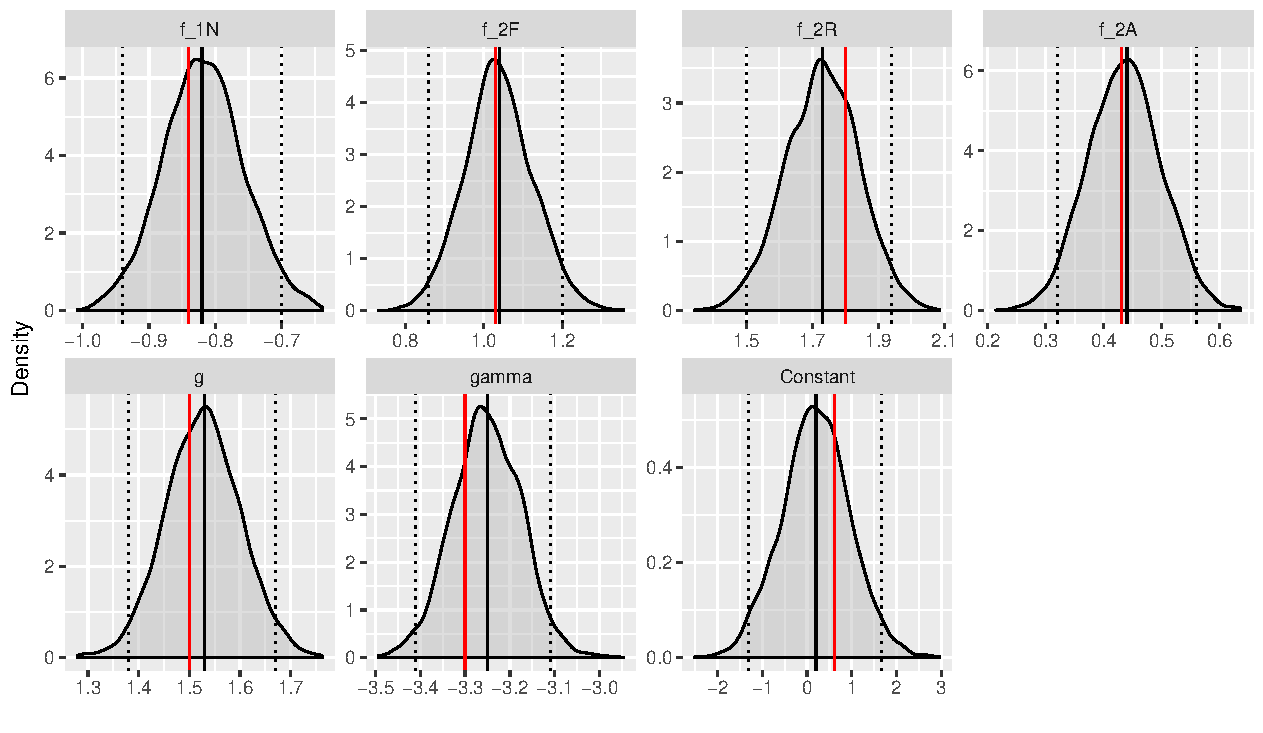
\includegraphics[width=\linewidth]{mkt3_v1n_SCOTYORK_post.pdf}
\caption{Posterior density function of elasticities w.r.t $V_{1N}$ - Market 3}
\label{fig:mkt3_v1n_SCOTYORK_post}
\caption*{Source: Own work}
\end{figure} 

% 3a.
With respect to the $V_{1N}$ demand, Figure \ref{fig:mkt3_v1n_SCOTYORK_post}, half of the coefficients had HDI's amplitude below 0.30 - $f_{1N}$, $g$ and $\gamma$, and half were above this value - $f_{2F}$, $f_{2R}$ and $\gamma$, achieving up to 0.43. Detailed information of the HDI is presented in the Appendix \ref{apd:bayes_hdi}. 

% 3bc
As one may notice, for this estimation, there were no discrepancies between the OLS mean estimates and the Bayesian ones - all were very close. This may have occurred because the OLS estimates have already had correct algebraic signs. Therefore, the constraints applied to the prior did not represent actually barriers to help to shape the posterior distributions. Indeed, there were no sharp edges in any distribution. 

Since the constraint was not effective, the priors become simply non-informative priors, and because of the large number of observations, the likelihood prevails, causing the estimation to be similar to the OLS. Indeed, all OLS estimates are lying inside the HDI interval.

The inefficiency of the prior may also explain the large standard deviations. As one may recover from Chapter \ref{chp:lit-rev}, in the presence of high correlation of variables, strong priors are important because defining the boundaries of one covariant automatically shapes the correlated one. Thus, the mixed and blurred joint effect of two correlated variables takes a cut-off point.

\begin{figure}[H]
\centering
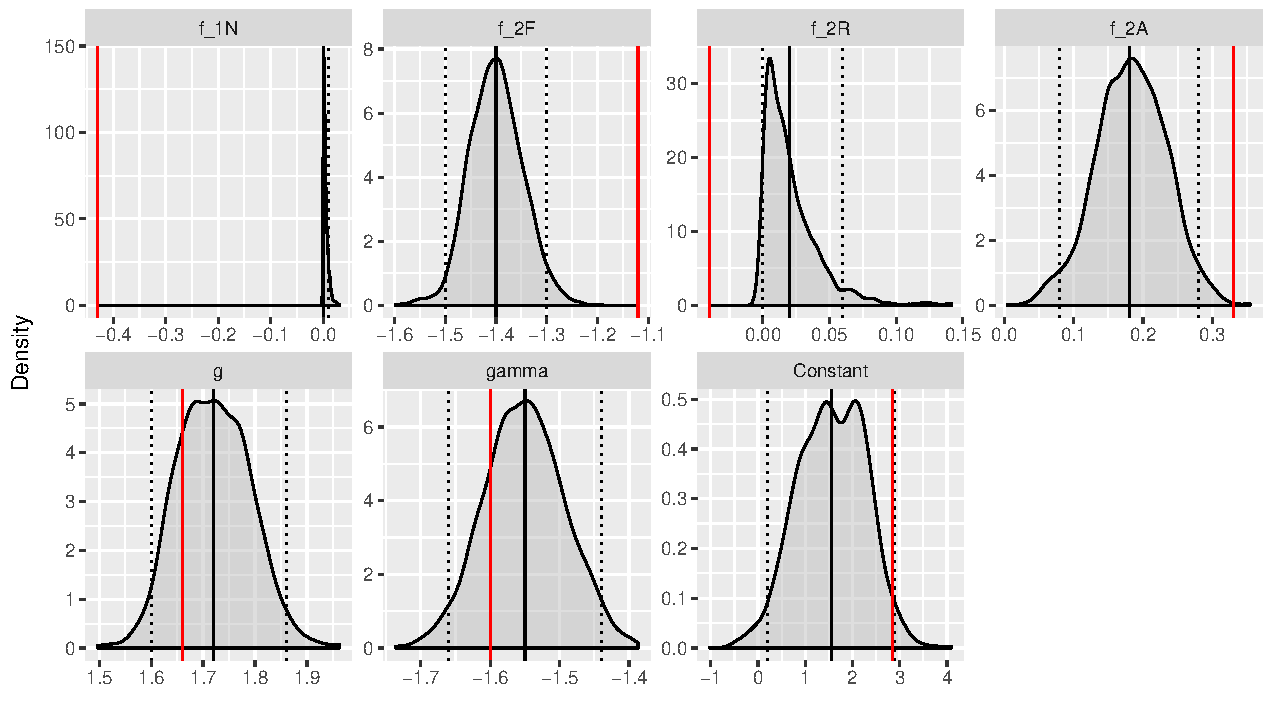
\includegraphics[width=\linewidth]{mkt3_v2f_SCOTYORK_post.pdf}
\caption{Posterior density function of elasticities w.r.t $V_{2F}$ - Market 3}
\label{fig:mkt3_v2f_SCOTYORK_post}
\caption*{Source: Own work}
\end{figure} 

% 3a
With respect to the $V_{2F}$ demand, Figure \ref{fig:mkt3_v2f_SCOTYORK_post}, the elasticities' HDI were satisfactorily small. The sign-reversed coefficients $f_{1N}$ and $f_{2N}$notably presented HDI with very small amplitude, 0.01 and 0.06, respectively. Detailed information of the HDI is presented in the Appendix \ref{apd:bayes_hdi}. 

% 3b
With these short HDI intervals, the OLS estimates lied out of the range of credible values for all estimates, but $g$. This shows that the precision of bayesian estimates was enough to distinguish even OLS estimates that already have correct algebraic signs from being credible values.

% 3c
It is noticeable that, once again, for the sign-reversed coefficients, the shape of the posterior distribution is skewed towards the zero value, showing that the imposition of constraint was fundamental to avoid the wrong sign estimates indicated by the likelihood.

% 3a
With respect to the $V_{2R}$ demand, Figure \ref{fig:mkt3_v2r_SCOTYORK_post}, the elasticities' HDI were again satisfactorily small. It is noticeable that, as in the previous model, the $f_{1N}$ elasticity was very close to zero HDI's range of 0.02. Detailed information of the HDI is presented in the Appendix \ref{apd:bayes_hdi}. 

% 3b
The OLS estimates lied out of the credible values of for $g$ and $\gamma$, besides the sign-reversed coefficients, for which it should already be expected. 

% 3c
Also, similarly to the last model, the sign-reversed coefficients had skewed distributions towards the zero constraints. A similar interpretation is applicable in this regard.

\begin{figure}[H]
\centering
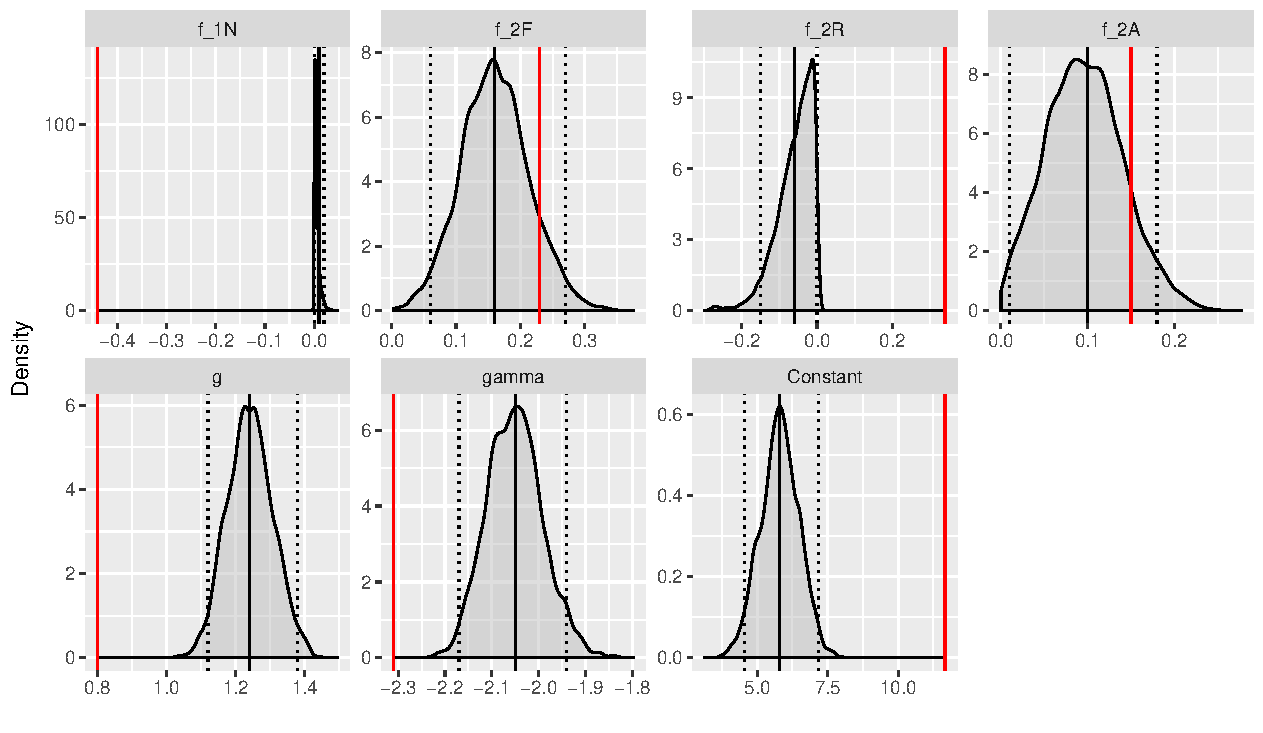
\includegraphics[width=\linewidth]{mkt3_v2r_SCOTYORK_post.pdf}
\caption{Posterior density function of elasticities w.r.t $V_{2R}$ - Market 3}
\label{fig:mkt3_v2r_SCOTYORK_post}
\caption*{Source: Own work}
\end{figure} 

\begin{figure}[H]
\centering
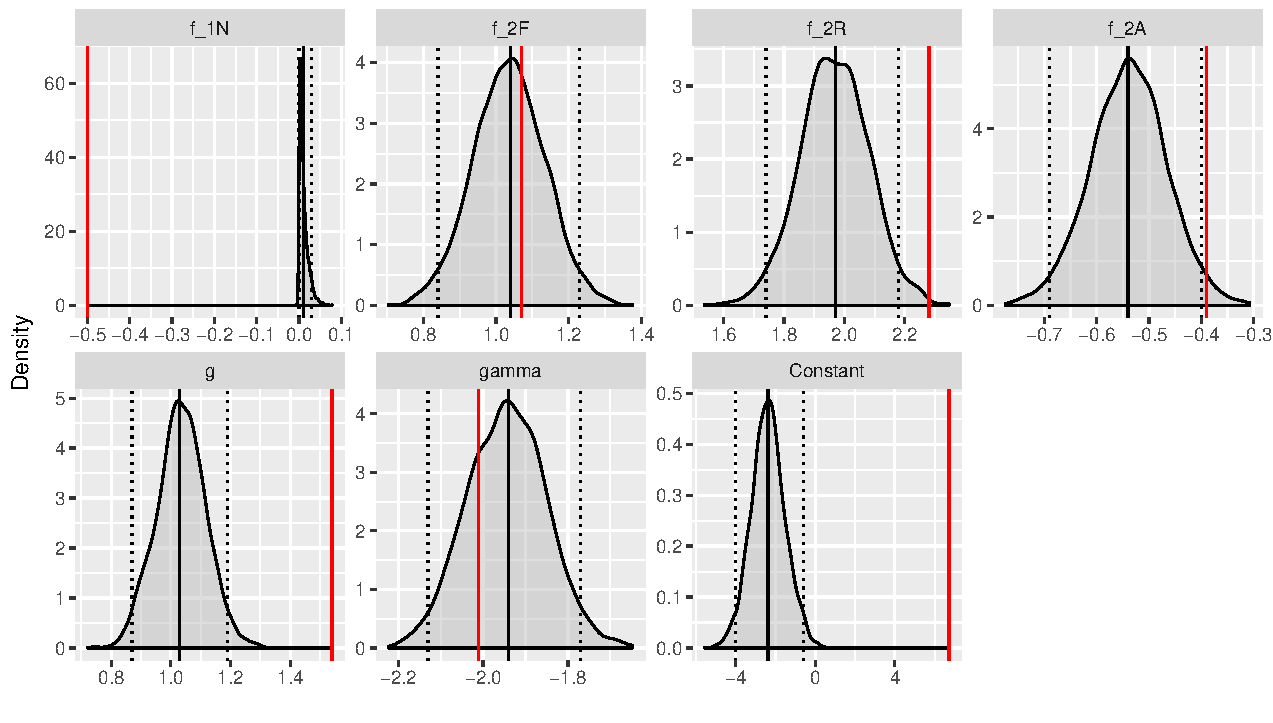
\includegraphics[width=\linewidth]{mkt3_v2a_SCOTYORK_post.pdf}
\caption{Posterior density function of elasticities w.r.t $V_{2A}$ - Market 3}
\label{fig:mkt3_v2a_SCOTYORK_post}
\caption*{Source: Own work}
\end{figure} 

% 3a
With respect to the $V_{2A}$ demand, Figure \ref{fig:mkt3_v2a_SCOTYORK_post}, the HDI are again presenting ranges above 0.30 up to 0.44 ($f_{2R}$). excepted for $f_{1N}$ and $f_{2A}$. The $f_{2A}$ was at the edge, with 029. Conversely, it is noticeable that the $f_{1N}$, as in the last model, it presented a very short HDI of 0.03. Detailed information of the HDI is presented in the Appendix \ref{apd:bayes_hdi}. 

% 3b
Even though the large HDI intervals, the OLS estimates lied out of the credible values for the $f_{1N}$, which was already expected since the OLS estimates were in the wrong domain, $f_{2R}$, $f_{2A}$ and $g$. 

% 3c
Once again, the sign-reversed coefficient had skewed distributions towards the zero constraints. A similar interpretation is applicable in this regard.
\\[3pt]

\textit{iv. Magnitude of estimates}

% 1.
Analysing the magnitude of coefficients, the most sensitive fare with regard its own price is the \textit{Full}, with mean -1.4, followed by the \textit{First Class}, with mean -0.82, \textit{Advance}, with mean -0.46 and \textit{Reduced}, with a very low mean of -0.06. Notably, the \textit{Full} fare remains very elastic in this market.

% 2.
Regarding the cross elasticities, there were very extreme values - small effects very close to zero and high cross elasticities, bigger than 1. 

Some notable observations deserves to be highlighed: the virtually null cross elasticities for the \textit{First Class} for all demands; the high cross elasticities of the \textit{Full} fare with respect to \textit{First Class} and \textit{Advance}, 1.04 for both and the also high effects of the \textit{Reduced} fare with respect to the \textit{First Class} and \textit{Advanced} demands - 1.73 and 1.97, respectively. That may deserve further investigation. Eventually other constraints may be applied to test the propability of these elasticities being smaller.

% 3.
The GVA elasticity was above unit for all type of demands, which may be deemed reasonable since PDFH states a general expected value of 1.1 \citep[p.~9, Chapter B1]{pdfhv5} and also considers that ``the elasticities to GDP (...) can be expected to vary by ticket type" \citep[p.~7, Chapter B2]{pdfh}. It worths noticing that $g_{2F} > g_{2R}$, which is consistent with the fact that the percentage of business journeys is higher in \textit{Full} tickets. However, it is intriguing that $g_{1N} < g_{2F}$ because \textit{First class} is usually associated with business journeys. Nevertheless, it should be highlighted that the 1N fare aggregates \textit{Full}, \textit{Reduced} and \textit{Advance} tickets from the first class. In other words, 1N mixes the types of fares for which PDFH have stated the shares of trip purposes - there is only differentiation of trip purpose between \textit{Full} and \textit{Reduced}, making it unclear to judge the elasticity magnitude by this terms.

% 4.
For the GJT effects, the elasticities were considerably high:  from -1.55, for the \textit{Full} demand, to -3.25, for the \textit{First Class}. Even though there is the same GVA's reservation that states that elasticities can be expected to vary by ticket type \citep{pdfh}, it is markedly above general interval expected by PDFH - -0.7 to -1.1 \citep{pdfhv5}. 

It is remarkable that the most quality sensitive fare is the \textit{First Class}, which is reasonable since the first class is a quality differentiation, but the relative magnitude of the others are difficult to interpret.

% ==================================
% ==================================
% ==================================

\subsection{Market 4}

\textit{i. Autocorrelation and convergence}

The estimation was complex again, as it was in the third. Except for the $V_{2R}$, the models demanded longer iterations (10,000 instead of 2,000) to converge with an acceptable amount of effective samples. Additionally, to reduce autocorrelation, the thinness was increased to 5 for $V_{1A}$ and $V_{2F}$. Nevertheless, the estimation was successful, as demonstrated by the statistics in Table \ref{mkt4_T_autocorr_convergence_SCOTYORK}.

As in all previous markets, there also were divergent transitions reported in all regressions of Market 4. The previous interpretation applies.

% latex table generated in R 3.3.2 by xtable 1.8-2 package
% Sat Aug  5 10:10:51 2017
\begin{table}[H]
\caption{Autocorrelation and Convergence Measures - Market 4}
\label{mkt4_T_autocorr_convergence_SCOTYORK}
\centering
\begin{tabular}{lrrrrrrrrrrrrrrrrrrrr}
\toprule 
 & \multicolumn{17}{c}{\textit{Dependent variable:}} \\ 
\cline{2-21} 
\\[-1.8ex] & \multicolumn{2}{c}{$ln \; V_{1F}$} & & \multicolumn{2}{c}{$ln \; V_{1R}$} & & \multicolumn{2}{c}{$ln \; V_{1A}$} & & \multicolumn{2}{c}{$ln \; V_{2F}$} & & \multicolumn{2}{c}{ $ln \; V_{2R}$} & &  \multicolumn{2}{c}{ $ln \; V_{2A}$}\\ 
\cline{2-3} \cline{5-6} \cline{8-9} \cline{11-12} \cline{14-15} \cline{17-18}
 & $\hat{R}$ & $n_{\text{eff}}$ & & $\hat{R}$ & $n_{\text{eff}}$  & & $\hat{R}$ & $n_{\text{eff}}$ & & $\hat{R}$ & $n_{\text{eff}}$ & & $\hat{R}$ & $n_{\text{eff}}$ & & $\hat{R}$ & $n_{\text{eff}}$\\  
\hline \\[-1.8ex] 
  $f_{1F}$ & 1.0 & 707 & & 1.0 & 373 & & 1.0 & 622 & & 1.0 & 173 & & 1.0 & 98 & & 1.0 & 408 \\
  $f_{1R}$ & 1.0 & 534 & & 1.0 & 273 & & 1.0 & 548 & & 1.0 & 186 & & 1.0 & 339 & & 1.0 & 473 \\
  $f_{1A}$ & 1.0 & 663 & & 1.0 & 409 & & 1.0 & 632 & & 1.0 & 139 & & 1.0 & 225 & & 1.0 & 435 \\
  $f_{2F}$ & 1.0 & 826 & & 1.0 & 260 & & 1.0 & 739 & & 1.0 & 147 & & 1.0 & 278 & & 1.0 & 515 \\
  $f_{2R}$ & 1.0 & 668 & & 1.0 & 308 & & 1.0 & 527 & & 1.0 & 133 & & 1.0 & 206 & & 1.0 & 284 \\
  $f_{2A}$ & 1.0 & 251 & & 1.0 & 354 & & 1.0 & 799 & & 1.0 & 121 & & 1.0 & 213 & & 1.0 & 410 \\
  $g$      & 1.0 & 442 & & 1.0 & 311 & & 1.0 & 507 & & 1.0 & 95  & & 1.0 & 211 & & 1.0 & 221 \\
  $\gamma$ & 1.0 & 596 & & 1.0 & 292 & & 1.0 & 533 & & 1.0 & 149 & & 1.0 & 268 & & 1.0 & 320 \\
  Const. & 1.0 & 485 & & 1.0 & 280 & & 1.0 & 469 & & 1.0 & 103  & & 1.0 & 197 & & 1.0 & 404 \\
  \hline
  Iter     & \multicolumn{2}{c}{10,000} && \multicolumn{2}{c}{10,000} && \multicolumn{2}{c}{10,000} && \multicolumn{2}{c}{10,000} && \multicolumn{2}{c}{2,000} && \multicolumn{2}{c}{10,000}\\
  Thin     & \multicolumn{2}{c}{1} && \multicolumn{2}{c}{1} && \multicolumn{2}{c}{5} && \multicolumn{2}{c}{5} && \multicolumn{2}{c}{1} && \multicolumn{2}{c}{1}\\
   \bottomrule
\end{tabular}
\caption*{Source: Own work}
\end{table}

\vspace{-2em}
\textit{ii. OLS comparison}

A comparison between the Bayes and OLS estimates is presented in Table \ref{tbl:mkt4_T_SCOTYORK}. As expected, all Bayesian coefficients have coherent signs. It clearly improved the estimates, reverting the ten wrong sign elasticities from the OLS estimates.
% \\[3pt]

\begin{landscape}
% latex table generated in R 3.3.2 by xtable 1.8-2 package
% Mon Jul 31 09:29:49 2017
\begin{table} [H]
\caption{Comparison of bayesian and SURE/OLS estimates - Martket 4}
\label{tbl:mkt4_T_SCOTYORK}
\centering
\begin{tabular}{lrrrrrrrrrrrrr}
  \toprule 
 & \multicolumn{6}{c}{\textit{Bayes}} && \multicolumn{6}{c}{\textit{SURE/OLS}} \\ 
\cline{2-7} \cline{9-14} 
\\[-1.8ex] & $ln \; V_{1F}$ & $ln \; V_{1R}$ & $ln \; V_{1A}$ & $ln \; V_{2F}$ & $ln \; V_{2R}$ & $ln \; V_{2A}$ & & $ln \; V_{1F}$ & $ln \; V_{1R}$ & $ln \; V_{1A}$ & $ln \; V_{2F}$ & $ln \; V_{2R}$ & $ln \; V_{2A}$ \\ 
\hline \\[-1.8ex] 

$f_{1F}$ & -1.02  & 0.04   & 1.10   & 0.02   & 0.16   & 0.46   && -0.94   & \cellcolor{gray!25}-0.09$^{\dagger}$   & 1.20    & \cellcolor{gray!25}-0.50   & 0.01$^{\dagger}$    & 0.54 \\ 
         & (0.19) & (0.04) & (0.19) & (0.02) & (0.12) & (0.20) && (0.22)  & (0.27)  & (0.27)  & (0.20)  & (0.19)  & (0.26) \\ [0.08cm]
$f_{1R}$ & 0.05   & -0.49  & 0.02   & 0.01   & 0.21   & 0.03   && 0.06$^{\dagger}$    & -0.43   & \cellcolor{gray!25}-0.25   & \cellcolor{gray!25}-0.14   & 0.22    & \cellcolor{gray!25}-0.11 \\ 
         & (0.04) & (0.07) & (0.02) & (0.01) & (0.05) & (0.03) && (0.06)  & (0.08)  & (0.08)  & (0.06)  & (0.05)  & (0.07) \\ [0.08cm]
$f_{1A}$ & 0.24   & 0.02   & -0.09  & 0.04   & 0.39   & 0.80   && 0.28    & \cellcolor{gray!25}-0.99   & \cellcolor{gray!25}0.09$^{\dagger}$    & \cellcolor{gray!25}0.33    & 0.44    & 0.88 \\ 
         & (0.11) & (0.02) & (0.07) & (0.03) & (0.09) & (0.13) && (0.125) & (0.151) & (0.154) & (0.114) & (0.108) & (0.147) \\ [0.08cm]
$f_{2F}$ & 0.91   & 0.46   & 0.72   & -1.04  & 0.45   & 0.83   && 0.85    & 0.71    & 0.74    & \cellcolor{gray!25}-0.59   & 0.51    & 0.82 \\ 
         & (0.13) & (0.13) & (0.16) & (0.09) & (0.12) & (0.16) && (0.15)  & (0.18)  & (0.18)  & (0.14)  & (0.13)  & (0.17) \\ [0.08cm]
$f_{2R}$ & 0.87   & 0.13  & 0.43   & 0.05   & -1.32  & 0.64   && 0.67    & 0.00$^{\dagger}$    & 0.10$^{\dagger}$    & \cellcolor{gray!25}-0.32$^{\dagger}$   & -1.32   & 0.46$^{\dagger}$ \\ 
         & (0.22) & (0.10) & (0.23) & (0.04) & (0.19) & (0.26) && (0.27)  & (0.33)  & (0.34)  & (0.25)  & (0.23)  & (0.32) \\ [0.07cm]
$f_{2A}$ & 0.16   & 1.28   & 0.82   & 0.04   & 0.31   & -1.08  && 0.18$^{\dagger}$    & 2.37    & 1.04    & 0.03$^{\dagger}$    & 0.35    & -0.99 \\ 
         & (0.12) & (0.17) & (0.19) & (0.03) & (0.14) & (0.20) && (0.18)  & (0.22)  & (0.22)  & (0.16)  & (0.16)  & (0.21) \\ [0.07cm]
$g$      & 1.91   & 1.21   & 0.69   & 2.37   & 1.87   & 1.30   && 2.74    & 1.17    & 1.12    & 2.86    & 1.91    & 1.86 \\ 
         & (0.09) & (0.17) & (0.10) & (0.08) & (0.08) & (0.09) && (0.18)  & (0.22)  & (0.22)  & (0.17)  & (0.16)  & (0.22) \\ [0.07cm]
$\gamma$ & -2.66  & -1.48  & -2.18  & -2.14  & -2.07  & -2.05  && -2.39   & -1.79   & -2.03   & -1.71   & -2.07   & -1.90 \\ 
         & (0.13) & (0.15) & (0.16) & (0.10) & (0.12) & (0.16) && (0.15)  & (0.18)  & (0.18)  & (0.14)  & (0.13)  & (0.18) \\[0.07cm]
Constant & -2.40  & -0.71  & -0.84  & -2.27  & -0.01  & -1.17  && -11.98  & -3.34$^{\dagger}$   & -5.89   & -8.38   & -0.38$^{\dagger}$   & -7.47 \\ 
         & (0.89) & (0.92) & (0.94) & (0.79) & 0.81   & (0.04) && (2.09)  & (2.53)  & (2.57)  & (1.91)  & (1.80)  & (2.46) \\ 
\bottomrule
\multicolumn{3}{l}{Note: $^{\dagger}$ $p>0.1$}
\end{tabular}
\caption*{Source: Own work}
\end{table}

\cellcolor{gray!25}
\end{landscape}

\textit{iii. Uncertainty}

% 1.
Figures \ref{fig:mkt4_v1f_SCOTYORK_post}, \ref{fig:mkt4_v1r_SCOTYORK_post}, \ref{fig:mkt4_v1a_SCOTYORK_post}, \ref{fig:mkt4_v2f_SCOTYORK_post}, \ref{fig:mkt4_v2r_SCOTYORK_post} and \ref{fig:mkt4_v2a_SCOTYORK_post} illustrate the probability densities of the estimated elasticities coefficients. The elements in the graphs remain as previously explained. 

% 2.
As for Market 3, the estimation in Market 4 has not reported small standard deviations. Neither was the amplitude of HDI intervals: for 35 out of 48 elasticities coefficients it was above 0.30. Once again, it worths highlight that there is always a trade-off between the precision of the HDI interval and the probability mass covered, which may be useful for practical applications.

\begin{figure}[H]
\centering
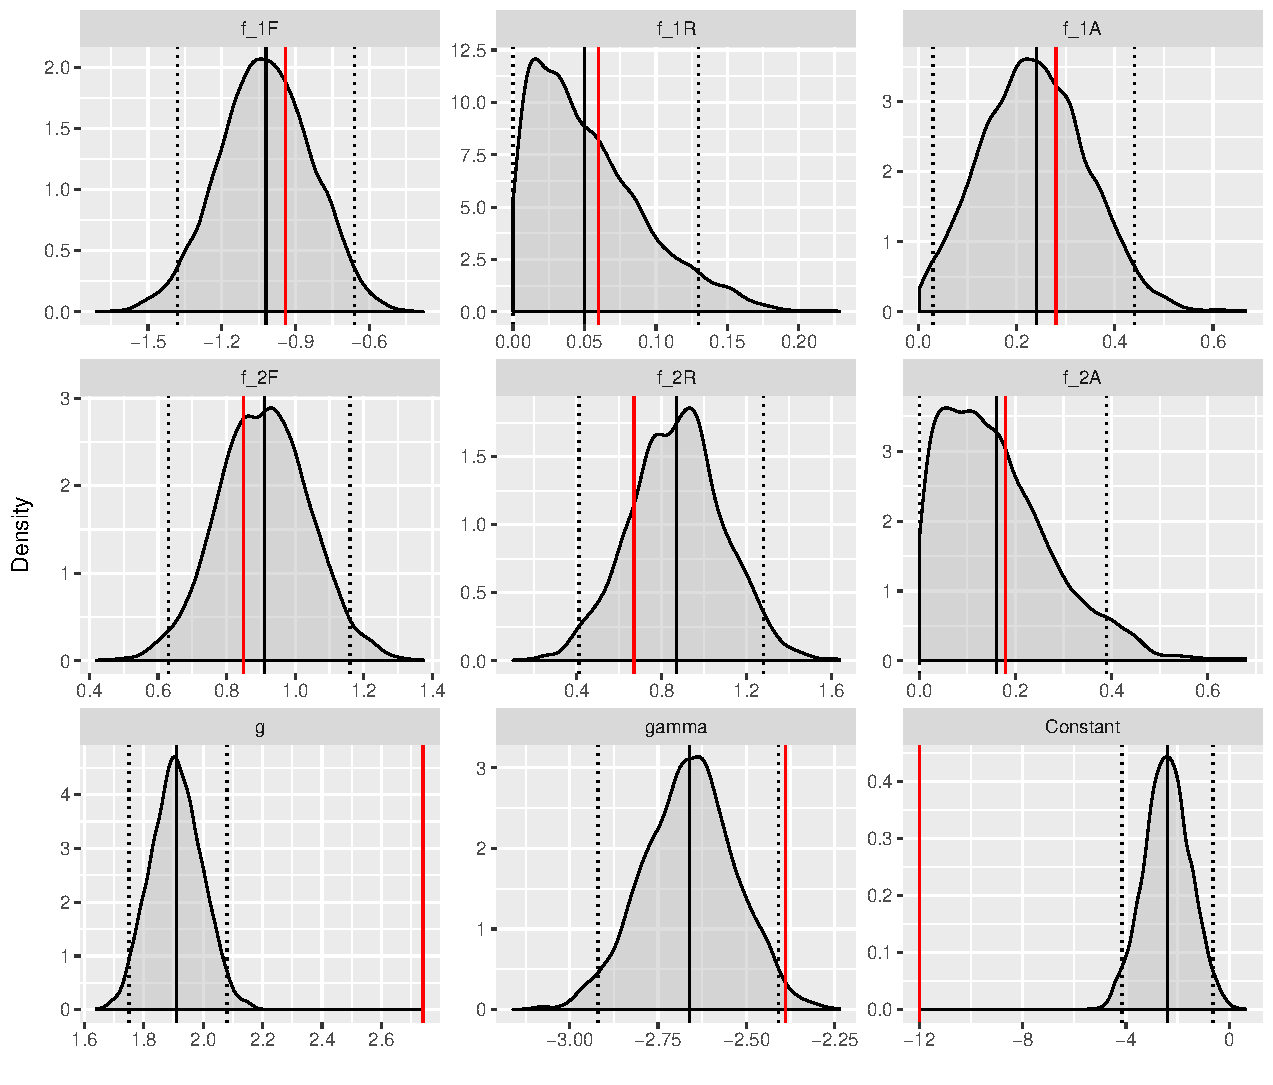
\includegraphics[width=\linewidth]{mkt4_v1f_SCOTYORK_post.pdf}
\caption{Posterior density function of elasticities w.r.t $V_{1F}$ - Market 4}
\label{fig:mkt4_v1f_SCOTYORK_post}
\caption*{Source: Own work}
\end{figure} 

% 3a
With respect to $V_{1F}$ demand, Figure \ref{fig:mkt4_v1f_SCOTYORK_post}, the only elasticity with short HDI was the $f_{1R}$, which amplitude is 0.13. For all others coefficients, the HDI range was significantly high. Detailed information of the HDI is presented in the Appendix \ref{apd:bayes_hdi}. 

% 3c
What happened in this estimation was similar to the $V_{1N}$ demand, in Market 3. The prior constraints had no effect on the likelihood and became non-informative priors since the OLS estimates already had correct signs. 

Nevertheless, two exceptions can be commented on that. It is noticeable that both $f_{1R}$ and $f_{2A}$ have an abrupt cut-off at zero, which may show that even though the mean value of OLS estimates already have correct signs, they were spreading to unfeasible values, which was cut by the prior constraint. Therefore, even though, the prior has not directly affected the mean value, it had a soft pressure in the distribution as a whole. 

% 3b
That, however, appears to be a weak pressure given the large standard deviations resulting and estimates to similar to the OLS, as explained in Market 3. Except by the $g$ and $\gamma$, all OLS estimates are lying inside the HDI interval.

\begin{figure}[H]
\centering
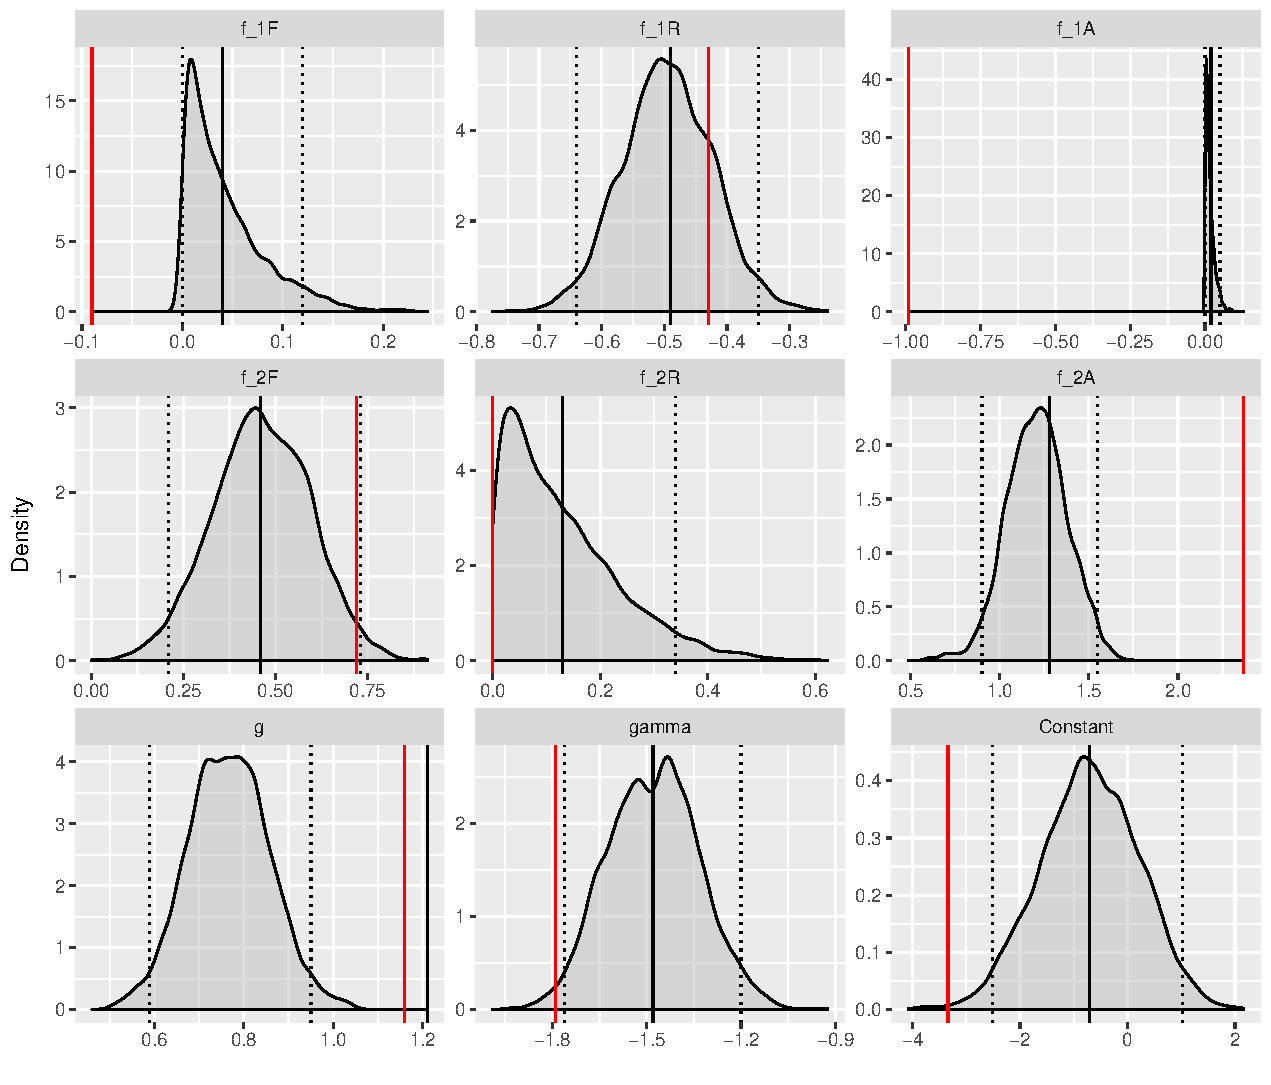
\includegraphics[width=\linewidth]{mkt4_v1r_SCOTYORK_post.pdf}
\caption{Posterior density function of elasticities w.r.t $V_{1R}$ - Market 4}
\label{fig:mkt4_v1r_SCOTYORK_post}
\caption*{Source: Own work}
\end{figure} 

% 3a
With respect to $V_{1R}$ demand, Figure \ref{fig:mkt4_v1r_SCOTYORK_post}, three elasticities presented satisfactorily small HDI: $f_{1F}$, $f_{1R}$ and $f_{1A}$, with 0.12, 0.29 and 0.05, respectively. It's noticeable that the shortest interval was the one from the sign-reversed elaticities, $f_{1F}$ and $f_{1A}$. For all others, it was above 0.30, up to 0.65 for the $f_{2R}$ elasticity. Detailed information of the HDI is presented in the Appendix \ref{apd:bayes_hdi}. 

% 3b
Even though the large HDIs, it was possible to distinguish the bayesian from OLS estimates: in addition to the sign-reversed coefficient, which should already be expected, the OLS lied out of the HDI for $f_2A$, $g$ and $\gamma$.

% 3c
Similarly to previous estimations, some distributions are skewed towards the zero constraints with sharp edges. Analogous interpretation is applicable in this regard.

\begin{figure}[H]
\centering
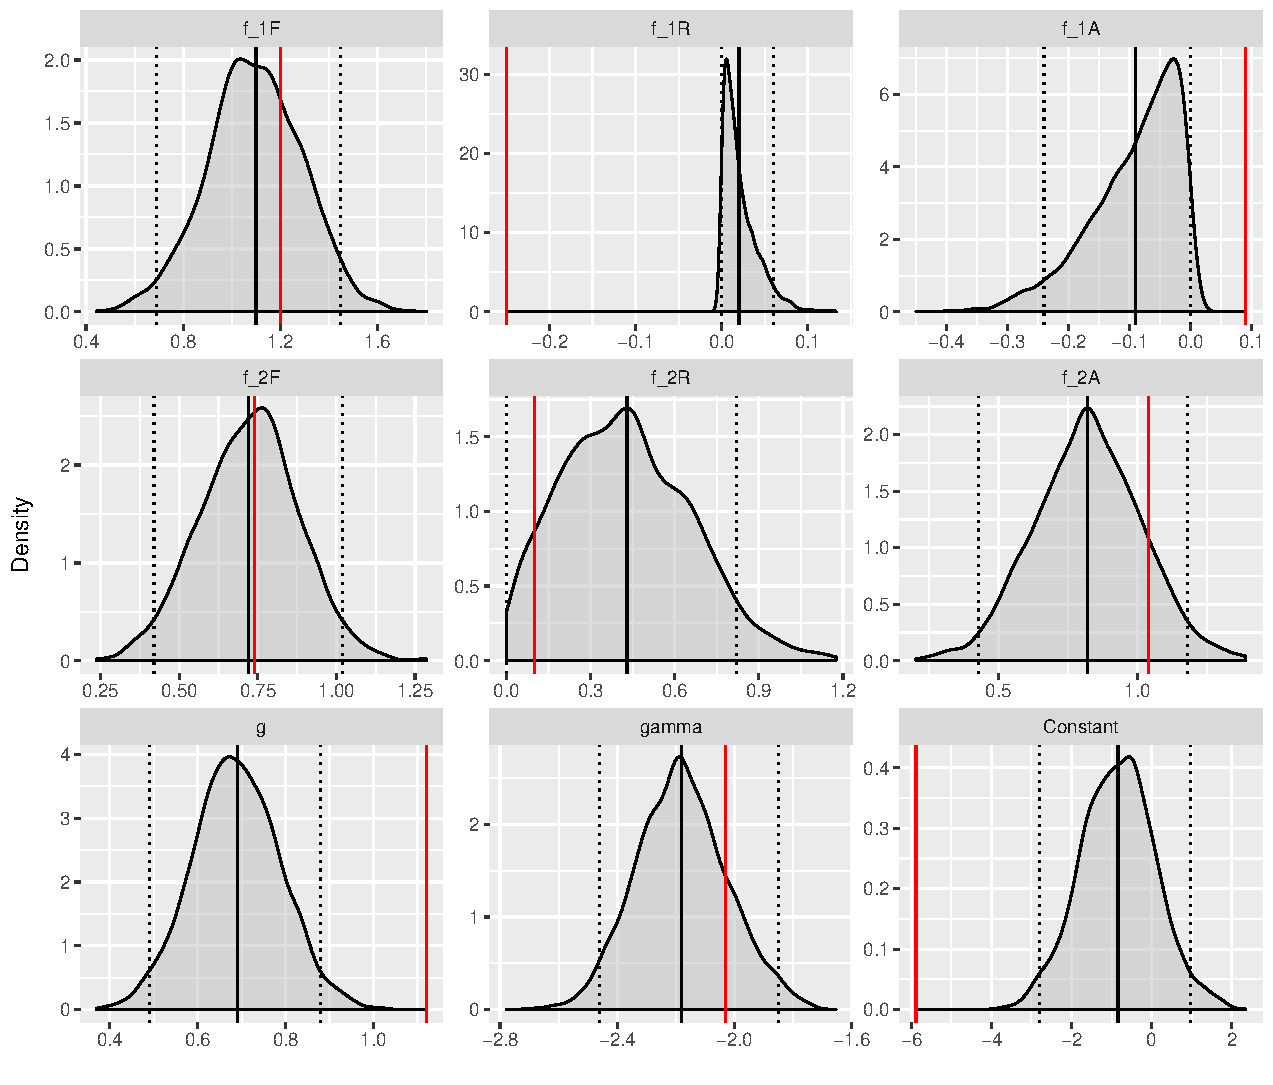
\includegraphics[width=\linewidth]{mkt4_v1a_SCOTYORK_post.pdf}
\caption{Posterior density function of elasticities w.r.t $V_{1A}$ - Market 4}
\label{fig:mkt4_v1a_SCOTYORK_post}
\caption*{Source: Own work}
\end{figure} 

% 3ac
With respect to $V_{1A}$ demand, Figure \ref{fig:mkt4_v1a_SCOTYORK_post}, only two elasticities presented short HDI's amplitude  - 0.06 for $f_{1R}$ and 0.24 for $f_{1A}$, which turn to be the constrained sign-reversed elasticities. Once again, skewness is observed and the sharp edge at zero has a similar interpretation from previous models. For all others coefficients, it was above 0.30, up to 0.82 for the $f_{2F}$. Detailed information of the HDI is presented in the Appendix \ref{apd:bayes_hdi}. 

% 3b
As it should be expected the OLS estimate lied out of the HDI for the sign-reversed elasticities. For all other elasticities, but $g$, the HDI was very large and the OLS estimates lied inside the range of 95\% probable values.

\begin{figure}[H]
\centering
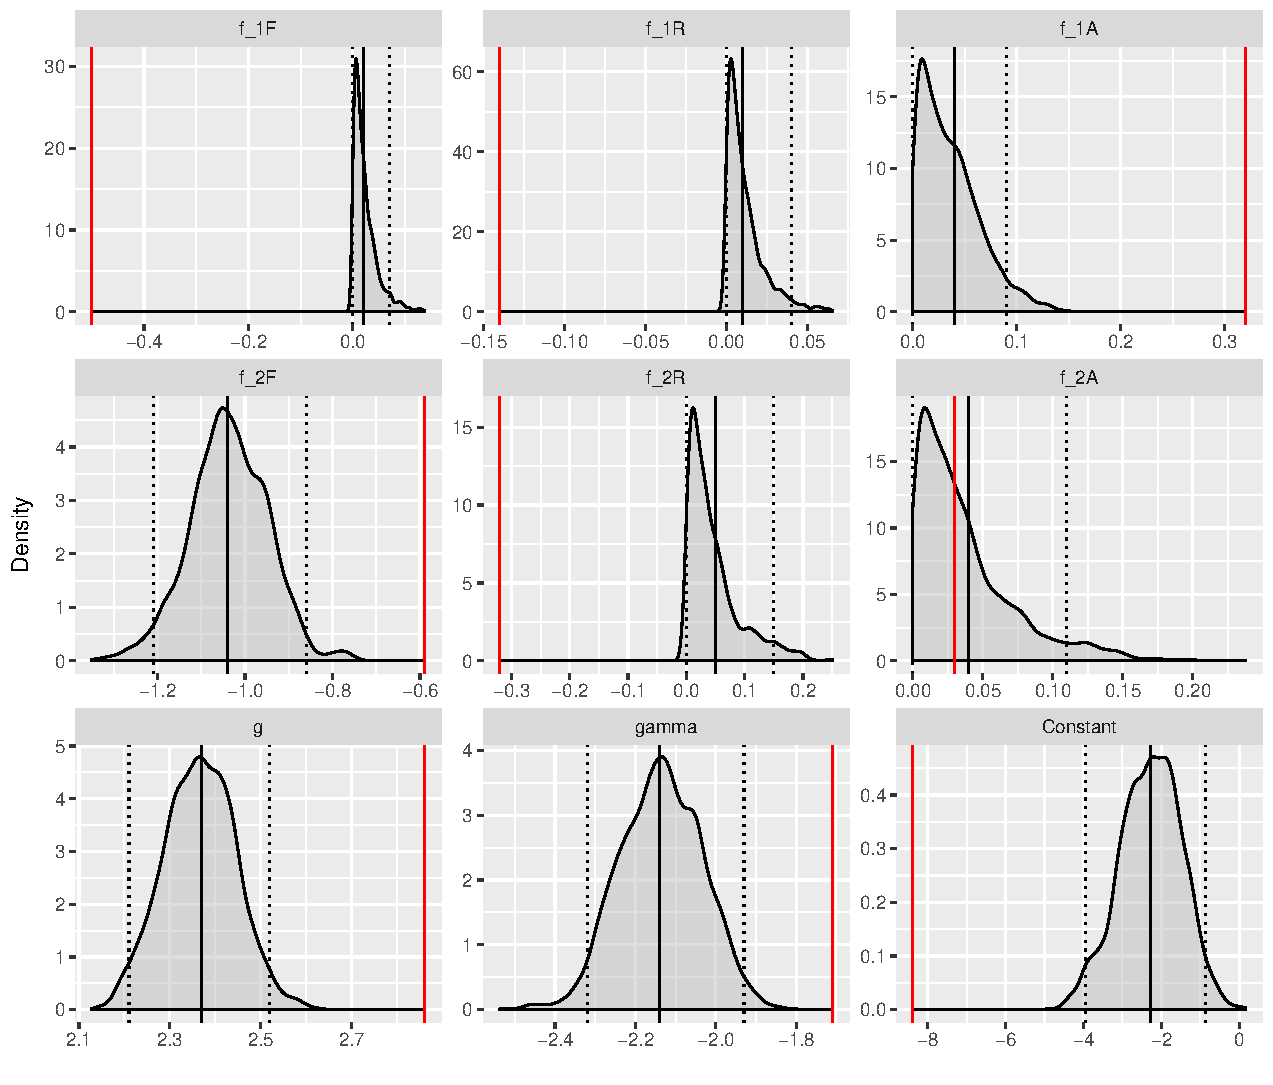
\includegraphics[width=\linewidth]{mkt4_v2f_SCOTYORK_post.pdf}
\caption{Posterior density function of elasticities w.r.t $V_{2F}$ - Market 4}
\label{fig:mkt4_v2f_SCOTYORK_post}
\caption*{Source: Own work}
\end{figure} 

% 3ac
The $V_{2F}$ model, Figure \ref{fig:mkt4_v2f_SCOTYORK_post}, was the estimation with the highest number of actual constraints. It is noticeable that the zero boundary was an actual barrier to the $f_{1F}$, $f_{1R}$, $f_{1A}$, $f_{2R}$ and $f_{2A}$ elasticities and these were the five OLS estimates wrong sign coefficients that were reverted in the Bayesian estimation.  With strong restrictions on the priors, the HDI was significantly shorter than in other estimations in this market, with five HDI ranging below 0.30. Even the ones higher 0.30 were around it, up to 0.38. Detailed information of the HDI is presented in the Appendix \ref{apd:bayes_hdi}. 

% 3b
Only the OLS elasticity of $f_{2A}$ lied inside the HDI interval, which demonstrates that squeezing the credible interval brought relevant information to the analysis.

\begin{figure}[H]
\centering
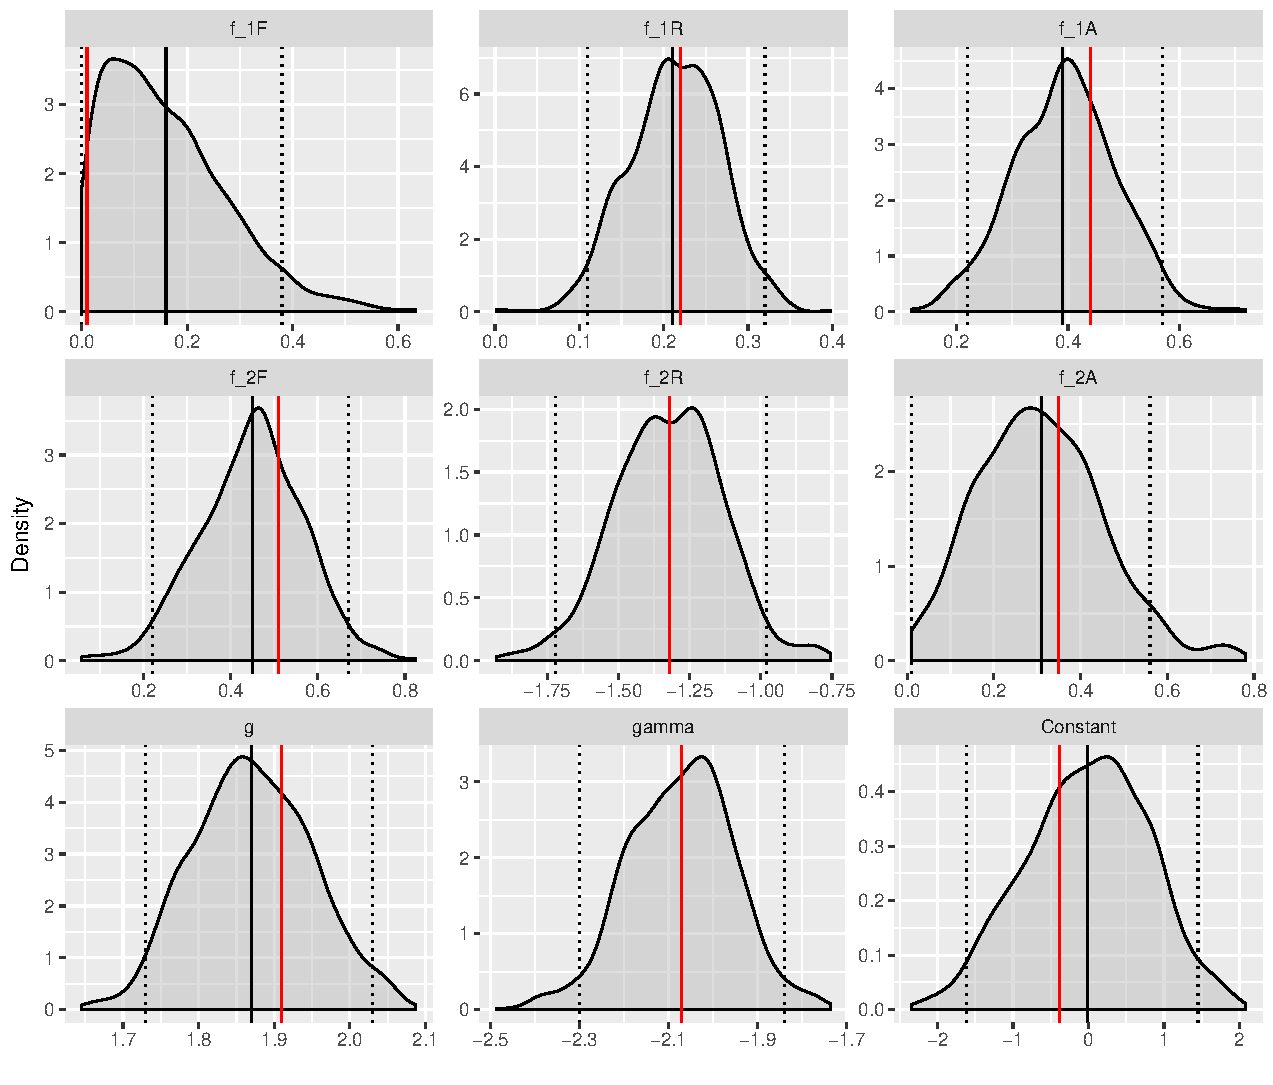
\includegraphics[width=\linewidth]{mkt4_v2r_SCOTYORK_post.pdf}
\caption{Posterior density function of elasticities w.r.t $V_{2R}$ - Market 4}
\label{fig:mkt4_v2r_SCOTYORK_post}
\caption*{Source: Own work}
\end{figure} 

% 3a
The estimation of $V_2R$ demand, Figure \ref{fig:mkt4_v2r_SCOTYORK_post}, was very similar to the $V_{1F}$ since any OLS estimates have wrong-sign. As explained before, without strong constraints, the likelihood prevailed and so the difficulty to address the correlation problems. Analogous interpretation is applied in this regard. 

The result was, once more, very large HDI, which means high uncertainty in the estimated elasticities. Only the $f_{1R}$ coefficient had HDI lower than 0.30. 

% 3b
Given that, the resultant estimates were very similar to the OLS estimates - all of them were inside the HDI. Even the $f_{2R}$ had a coincident mean.

\begin{figure}[H]
\centering
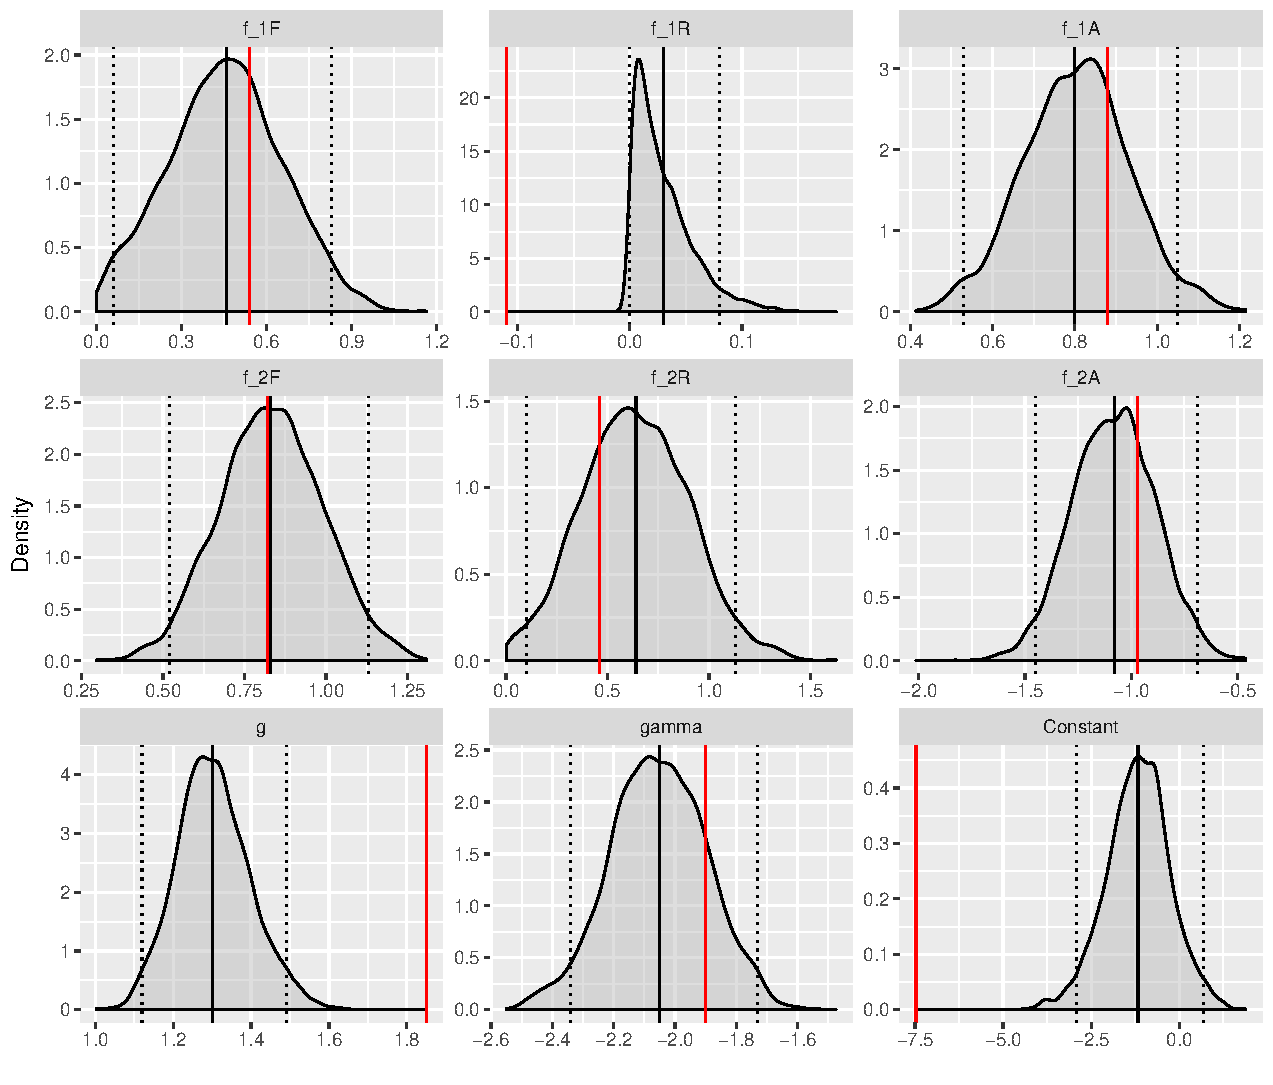
\includegraphics[width=\linewidth]{mkt4_v2a_SCOTYORK_post.pdf}
\caption{Posterior density function of elasticities w.r.t $V_{2A}$ - Market 4}
\label{fig:mkt4_v2a_SCOTYORK_post}
\caption*{Source: Own work}
\end{figure} 

% 3a
With respect to $V_2A$ demand, Figure \ref{fig:mkt4_v2a_SCOTYORK_post}, only the $f_{1R}$ elasticity suffered an actual constraint by the prior. As one may notice, it was, as usual, a wrong-sign OLS estimate reversed in the Bayesian estimation, resulting in a skewed distribution towards its boundaries. 

It appears, however, that because it is a very complex model, this was not enough to shape the other variables since all of HDI remained very large, up to 1.02. Once again, OLS lied inside the HDI, which makes one consider them as credible values, except for the $f_{1R}$, which should already be expected since it is the reversed coefficient, and the $g$ elasticities.
\\[3pt]

\textit{iv. Magnitude of estimates}

% % 0.
% Recognising that the interpretation of the estimates magnitude demands a deeper investigation of the rail market, demands support of  For that reason, the following considerations are mostly general aspects.

% 1.
Analysing the magnitude of coefficients, the most sensitive fare with regard its own price is the \textit{Standard Reduced}, with mean -1.32, followed by the \textit{Standard Advance}, \textit{Standard Full} and \textit{First Class Full}, with almost proportional effects - -1.08, -1.04 and -1.02, respectively. Smaller own elasticities were observed for the other \textit{First Class}, -0.51 and -0.09, which suggests less elastic demands. These values are considerably different from Market 3.

% 2.
Regarding to the cross elasticities, the \textit{First Class Full} fare has very small - almost null - price effects in the demand of the \textit{First Class Reduced} and \textit{Standard Full}, 0.02 and 0.05, respectively. Higher impacts, but still less than proportional occur in the demand of \textit{Standard Reduced} and \textit{Standard Advance}, 0.16 and 0.46, respectively. The \textit{First Class Advance} is surprisingly high, with 1.10, suggesting that, for first class passengers, the \textit{Advance} demand is very sensitive to changes in the \textit{Full} fare. This may sign there is a cost for passengers to plan their trips in advance.

For the \textit{First Class Reduced}, the most significant cross elasticities regarded the impact in the $V_{2R}$ demand, 0.21, all the other were very close to zero.

For the \textit{First Class Advance}, the impact in the $V_{1R}$ and $V_{2F}$ demand was also very close to zero. Higher effects were observed impacting the \textit{First Class Full} and \textit{Standard Reduced}, being of 0.24 and 0.39, respectively. The highest impact regards the \textit{Standard Advance} demand, deemed as 0.80.

Conversely, the \textit{Standard Full} have not presented such small cross elasticities. The smallest one regarding the impact in the \textit{Standard Reduced} demand, comparable to the effect in the \textit{First Class Reduced}, deemed as 0.46. The highest impact was 0.91 with regard to the \textit{First Class Full} demand.

For the \textit{Standard Reduced}, the cross elasticities with respect to the \textit{First Class Reduced} and \textit{Standard Full} demand were the smallest, 0.13 and 0.05, respectively. The biggest effect is the impact in the \textit{First Class Full}, deemes as 0.87.

The \textit{Standard Advance} had a small cross effect with respect to the \textit{First Class Full} and \textit{Standar Full}, 0.16 and 0.04, respectively. A very high impact was observed for the \textit{First Class Reduced} 1.28 - even higher than the own elasticity.

Generally, cross elasticities have ranged for very small values, close to zero, to very high ones, above 1. It was not possible to understand the interaction pattern neither even why some cross elasticities are higher than the own-elasticity.

% 3.
The GVA elasticity it worths noticing that the $g_{F} > g_{R}$ for both \textit{First} and \textit{Standard Class}, which is consistent with the fact that the percentage of business journeys is higher in \textit{Full} tickets. Additionally, the \textit{Standard Class} elasticities are higher relative to the \textit{First Class}, which may suggest that increase in productivity impacts more the mass of medium level professionals relatively to the white collar professional, that demand first class services. 

% 4.
For the GJT effects, the elasticities were considerably high: from -1.42, for the \textit{First Class Reduced} demand, to -2.66, for the \textit{First Class}. Even though there is the same GVA's reservation that states that elasticities can be expected to vary by ticket type \citep{pdfh}, it is markedly above general interval expected by PDFH - -0.7 to -1.1 \citep{pdfhv5}.